\documentclass[a4paper,11pt,oneside]{book}

%%% το αρχείο αυτό καθορίζει το look που έχουν οι pythonies
%%% γίνεται \input από όλα τα κεφάλαια και τα φύλλα εργασίας

% χρησιμοποιούμενα πακέτα: 
% 
% polyglossia
% xstring
% graphicx
% caption
% xcolor
% hyperref
% minted
% geometry
% titlesec
% datetime
% changepage
% ntheorem

% οριζόμενες εντολές:
%
% smallcaps (βοηθ. removeaccents)
%    μικρά κεφαλαία χωρίς τόνους στα φωνήεντα
% scaling
%    η κλιμάκωση *όλων* των illustrations, τρέχουσα τιμή 0.9
% iconcomputer, iconkeyboard, icondiscuss, iconfillin, iconcaution, iconprompt, dottedline
%    εικονίδια για τα φύλλα εργασίας και εστιγμένη γραμμή
% marginnote
%    πλευρικό σχόλιο
% chapterwabstract (βοηθ. abstract, boxcolor, chaptercolor, concepts, tmpconcepts)
%    εισαγωγικό κείμενο κεφαλαίου με χρωματιστό τετράγωνο, συνοδευτικές έννοιες, κλπ.
% tobecontinued
%    εμφανίζει το "συνεχίζεται στην επόμενη σελίδα"

% οριζόμενα περιβάλλοντα:
% 
% note
%    μια υποσημείωση ή υπόδειξη, με μικρότερα γράμματα
% question
%    μια ερώτηση που "οδηγεί" κάθε νέα ενότητα
% answer
%    μια απάντηση σε μια ερώτηση του φύλλου εργασίας
% theory
%    μια ενότητα "θεωρίας" (στο τέλος ενός κεφαλαίου)
% exercise
%    μια αριθμημένη άσκηση
% step
%    ένα αριθμημένο βήμα (για φύλλο εργασίας)

% για μορφοποίηση κώδικα:
%
% pycode (περιβάλλον)
%     κώδικας python χωρίς αρίθμηση
% pyfile (εντολή)
%     εισαγωγή κώδικα python από αρχείο
% pyfilenl (εντολή)
%     εισαγωγή κώδικα python από αρχείο χωρίς αρίθμηση γραμμών
% pyfilesrc (εντολή)
%    εισαγωγή κώδικα από αρχείο με link στο αρχείο
% pyinline (εντολή)
%     κώδικας python μέσα στη ροή του κειμένου
% pyplain (περιβάλλον, για τα φύλλα εργασίας)
%     κώδικας python χωρίς φόντο
% pynew (περιβάλλον, για τα φύλλα εργασίας)
%     κώδικας python με φόντο
% pyterm (περιβάλλον για τα φύλλα εργασίας)
%     η είσοδος του χρήστη ή τα περιεχόμενα της οθόνης
% pyhighlight (εντολή)
%    highlight κειμένου (χρησιμοποιείται για κώδικα μέσα σε pyplain)


%%% επιλογές γλώσσας και γραμματοσειρών για το XeLaTeX

\usepackage{polyglossia}
\setdefaultlanguage{greek}
\setmainfont[Ligatures=TeX,SmallCapsFont={Linux Libertine O C},SmallCapsFeatures={Letters=SmallCaps}]{Linux Libertine O}
\setsansfont{Linux Biolinum O}
\setmonofont{Ubuntu Mono}
\enablehyphenation

% αφαίρεση τόνων από τα smallcaps
\usepackage{xstring}
\newcommand{\removeaccents}[1]{%
\def\result{#1}%
\StrSubstitute{\result}{ά}{α}[\result]%
\StrSubstitute{\result}{έ}{ε}[\result]%
\StrSubstitute{\result}{ή}{η}[\result]%
\StrSubstitute{\result}{ί}{ι}[\result]%
\StrSubstitute{\result}{ό}{ο}[\result]%
\StrSubstitute{\result}{ύ}{υ}[\result]%
\StrSubstitute{\result}{ώ}{ω}[\result]%
\StrSubstitute{\result}{Ά}{Α}[\result]%
\StrSubstitute{\result}{Έ}{Ε}[\result]%
\StrSubstitute{\result}{Ή}{Η}[\result]%
\StrSubstitute{\result}{Ί}{Ι}[\result]%
\StrSubstitute{\result}{Ό}{Ο}[\result]%
\StrSubstitute{\result}{Ύ}{Υ}[\result]%
\StrSubstitute{\result}{Ώ}{Ω}[\result]%
\result
}

\newcommand{\smallcaps}[1]{\textsc{\removeaccents{#1}}}

%%% εικόνες και λεζάντες

\usepackage{graphicx}
\newcommand{\scaling}{0.9}
\usepackage{caption}
\captionsetup{font=footnotesize}

%%% ειδικά περιβάλλοντα

\usepackage{xcolor}

% ερωτήσεις (που οδηγούν στην επόμενη ενότητα)
\definecolor{questioncolor}{rgb}{0.6,0.5,0.5}
\newenvironment{question}{\noindent\itshape\color{questioncolor}}{\noindent\ignorespaces}

% απαντήσεις (για τις ερωτήσεις των φύλλων εργασίας)
\definecolor{answercolor}{rgb}{0.5,0.5,0.5}
\newenvironment{answer}{\marginnote[16pt]{\iconfillin}\noindent\itshape\color{answercolor}}{\noindent\ignorespaces}

% περιβάλλον "θεωρίας" (πλήρες πλάτος κειμένου)
\usepackage{changepage}
\newenvironment{theory}[1]{\begin{adjustwidth}{}{-\overhang}\smallcaps{#1}\itshape}{\end{adjustwidth}}

% απομεινάρια...
% \newlength{\theoryrulelength}
% \setlength{\theoryrulelength}{36pt}
% \newenvironment{theory}{\rule{\theoryrulelength}{0.4pt}\begin{adjustwidth}{}{-\overhang}\itshape}{\end{adjustwidth}\rule{\theoryrulelength}{0.4pt}}

%%% υπερσύνδεσμοι

\definecolor{linkcolor}{rgb}{0.0,0.5,0.25}
\usepackage[colorlinks=true,urlcolor=linkcolor]{hyperref}

%%% εικονίδια και εστιγμένες γραμμές (για τα φύλλα εργασίας)

\newcommand{\iconcomputer}{
\includegraphics[scale=0.35]{../../share/circle-icons/one-color/computer.eps}}
\newcommand{\iconkeyboard}{
\includegraphics[scale=0.35]{../../share/circle-icons/one-color/keyboard.eps}}
\newcommand{\icondiscuss}{
\includegraphics[scale=0.35]{../../share/circle-icons/one-color/chat.eps}}
\newcommand{\iconfillin}{
\includegraphics[scale=0.35]{../../share/circle-icons/one-color/compose.eps}}
\newcommand{\iconcaution}{
\includegraphics[scale=0.35]{../../share/circle-icons/one-color/caution.eps}}
\newcommand{\iconprompt}{
\includegraphics[scale=0.35]{../../share/circle-icons/one-color/prompt.eps}}
\newcommand{\dottedline}{\vspace{\parskip}\dotfill}

%%% συνεχίζεται στην επόμενη σελίδα

\newcommand{\tobecontinued}{\mbox{}\hfill{\footnotesize ...συνεχίζεται στην επόμενη σελίδα.}}
\newenvironment{note}{\small\upshape}{}

%%% μορφοποίηση κώδικα με το pygmentize

\usepackage{minted}

% fix για ένα bug στο minted που εμφανίζεται όταν χρησιμοποιείται χρώμα στο φόντο (bgcolor)
% http://tex.stackexchange.com/questions/228058/how-to-space-before-and-after-a-minted-code-block-with-bgcolor
\makeatletter
\patchcmd{\minted@colorbg}{\noindent}{\noindent}{}{}
\apptocmd{\endminted@colorbg}{}{}{}
\makeatother

% χρώματα φόντου για τον κώδικα
\definecolor{codebg}{rgb}{0.80,0.95,0.85}
\definecolor{newcodebg}{rgb}{0.75,0.95,0.85}

% ορισμοί για τα περιβάλλοντα κώδικα
% pycode: περιβάλλον κώδικα python χωρίς αρίθμηση
\newminted[pycode]{python3}{bgcolor=codebg}
% pyfile: python από αρχείο
\newmintedfile[pyfile]{python3}{linenos=true,numberblanklines=false,escapeinside=||,bgcolor=codebg}
% pyfilenl: python από αρχείο χωρίς αρίθμηση γραμμών
\newmintedfile[pyfilenl]{python3}{linenos=false,numberblanklines=false,escapeinside=||,bgcolor=codebg}
% pyinline: python μέσα στη ροή του κειμένου
\newmintinline[pyinline]{python3}{linenos=true,numberblanklines=false}
% pyplain: (για τα φύλλα εργασίας) περιβάλλον χωρίς φόντο
\newminted[pyplain]{python3}{bgcolor=white,escapeinside=||,formatcom={\upshape}}
% pynew: (για τα φύλλα εργασίας) περιβάλλον με φόντο
\newminted[pynew]{python3}{bgcolor=newcodebg,escapeinside=||,formatcom={\upshape}}
% pyterm: (για τα φύλλα εργασίας) περιβάλλον για τα περιεχόμενα της οθόνης
\newminted[pyterm]{text}{bgcolor=white,escapeinside=||}

%\newminted[pyterm]{text}{escapeinside=||}
% [TODO] fix: το pyterm χωρίς bgcolor εμφανίζει μεγαλύτερα περιθώρια (πάνω και κάτω) και δεν φαίνεται ωραίο. Το bgcolor είναι προσωρινό workaround, έχει κι αυτό margins (για να μην είναι κολλητά ο κώδικας με το περιθώριο) κι έτσι ο κώδικας στ' αριστερά δεν είναι τέλεια στοιχισμένος.

% εντολή για κώδικα από αρχείο με link στο αρχείο
\newcommand{\pyfilesrc}[2][]{%
\pyfile[#1]{#2}\\
\mbox{}\hfill{\scriptsize\href{http://pythonies.mysch.gr/#2}{\url{#2}}}
}

% εντολή για το highlighting του κώδικα (συνήθως σε pyplain περιβάλλον με escapeinside)
\newcommand{\pyhighlight}[1]{\colorbox{newcodebg}{#1}}

%%% αριθμημένα περιβάλλοντα

\usepackage{ntheorem}

% άσκηση
\makeatletter
\theoremheaderfont{\upshape}%\upshape\bfseries\scshape}
\theorembodyfont{\itshape}%\slshape}
\newtheoremstyle{lmargin}%
  {\item[\theorem@headerfont \llap{##2}\hskip\labelsep\hskip-6pt]}%
  {\item[\theorem@headerfont \llap{##2}\hskip\labelsep ##1\ (##3)\theorem@separator]}
\makeatother
\theoremstyle{lmargin}
\newtheorem{exercise}{}[chapter]

% βήμα φύλλου εργασίας
\makeatletter
\theoremheaderfont{\bfseries}%\upshape\bfseries\scshape}
\theorembodyfont{\upshape}%\slshape}
\newtheoremstyle{lmarginup}%
  {\item[\theorem@headerfont \llap{##2}\hskip\labelsep\hskip-6pt]}%
  {\item[\theorem@headerfont \llap{##2}\hskip\labelsep ##1\ (##3)\theorem@separator]}
\newtheoremstyle{slmarginup}%
  {\item[\theorem@headerfont \llap{##1##2.}\hskip\labelsep\hskip-6pt]}%
  {\item[\theorem@headerfont \llap{##2.}\hskip\labelsep ##1\ (##3)\theorem@separator]}
\makeatother

% deprecated: \newcommand{\standalone}{} to define standalone
%\ifdefined\standalone
    \theoremstyle{slmarginup}
    \newtheorem{step}{}
%\else
%    \theoremstyle{lmarginup}
%    \newtheorem{step}{}[chapter]
%\fi

%%% γεωμετρία σελίδας και συναφείς ορισμοί από το tufte-latex
%%% https://tufte-latex.github.io/tufte-latex/

% εσοχή και διάστημα μεταξύ παραγράφων
% δεν επηρρεάζει το tufte-latex
\parindent=0pt
\parskip=6pt

% γεωμετρία σελίδας και ορισμός μηκών
\usepackage[a4paper,left=24.8mm,top=27.4mm,headsep=2\baselineskip,textwidth=107mm,marginparsep=8.2mm,marginparwidth=49.4mm,textheight=66\baselineskip,headheight=\baselineskip]{geometry}

\setlength{\marginparpush}{12pt}
\addtolength{\marginparpush}{\parskip}
\newlength{\fullwidth}
\setlength{\fullwidth}{\textwidth}
\addtolength{\fullwidth}{\marginparsep}
\addtolength{\fullwidth}{\marginparwidth}
\newlength{\overhang}
\setlength{\overhang}{\marginparsep}
\addtolength{\overhang}{\marginparwidth}

% απομεινάρια...
%\setlength\abovedisplayskip{6pt plus 2pt minus 4pt}
%\setlength\belowdisplayskip{6pt plus 2pt minus 4pt}

% italicize description run-in headings (instead of the default bold)
\renewcommand*\descriptionlabel[1]{\hspace\labelsep\normalfont\em #1}

% πλευρική σημείωση
\newcommand\marginnote[2][0pt]{%
  \marginpar{\hbox{}\vspace*{#1}\vspace*{-1\baselineskip}\noindent \footnotesize\textup{#2}}%
  {}%
}

% formatting title sections
\setcounter{secnumdepth}{-1}

\usepackage{titlesec}
\usepackage[nodate]{datetime}
\newlength{\beforesection}
\setlength{\beforesection}{3ex plus 0.5ex minus 0.2ex}
\addtolength{\beforesection}{-\parskip}
\newlength{\aftersection}
\setlength{\aftersection}{1.5ex plus 0.2ex}
\addtolength{\aftersection}{-\parskip}
\titlespacing*{\section}{0pt}{\beforesection}{\aftersection}

% απομεινάρια...
%\titlespacing*{\chapter}{0pt}{50pt}{40pt}
%\titlespacing*{\section}{0pt}{3.5ex plus 1ex minus .2ex}{2.3ex plus .2ex}

%%% για εισαγωγικό κείμενο κεφαλαίου με χρωματιστό τετράγωνο, συνοδευτικές έννοιες, κλπ.

\newcommand{\abstract}{}
\newcommand{\boxcolor}{}
\newcommand{\chaptercolor}{}
\newcommand{\concepts}{}
\newcommand{\tmpconcepts}{}
\newif\ifbonus

% reference: \titleformat{ command }[ shape ]{ format }{ label }{ sep }{ before-code }[ after-code ]
\titleformat{\chapter}[block]
{\Huge\sffamily}
{}
{0pt}
{\ifbonus\marginnote[-6pt]{\fcolorbox{\boxcolor}{\chaptercolor}{\makebox(40,40){\strut\textcolor{\boxcolor}{\Huge\thechapter}}}\\\vspace{\parskip}\\\tiny\today\\ \currenttime}\else\marginnote[-6pt]{\colorbox{\boxcolor}{\makebox(40,40){\strut\textcolor{\chaptercolor}{\Huge\thechapter}}}\\\vspace{\parskip}\\\tiny\today\\ \currenttime}\fi}
[\small\rmfamily\textmd\abstract\vspace{\parskip}\concepts\vspace{\parskip}\\\mbox{}\hrulefill]

\newcommand{\chapterwabstract}[5]{
	\renewcommand{\abstract}{#2}
    \renewcommand{\tmpconcepts}{#3}
	\ifdefempty{\tmpconcepts}{\renewcommand{\concepts}{}}{\renewcommand{\concepts}{\\\textbf{Έννοιες: }\tmpconcepts}}
	\renewcommand{\boxcolor}{#4}
	\renewcommand{\chaptercolor}{#5}
	\chapter{#1}
}

\definecolor{introColor}{rgb}{0.25,0.5,0.75}
\definecolor{answerColor}{rgb}{0.25,0.75,0.5}
\definecolor{crapsColor}{rgb}{0.5,0.75,0.25}
\definecolor{subtractionColor}{rgb}{0.5,0.25,0.75}
\definecolor{guessColor}{rgb}{0.75,0.25,0.5}
\definecolor{nimColor}{rgb}{0.75,0.5,0.25}
\definecolor{planetColor}{rgb}{0.25,0.25,0.75}
\definecolor{hangmanColor}{rgb}{0.25,0.75,0.25}
\definecolor{oxoColor}{rgb}{0.75,0.25,0.25}

\setcounter{part}{2}
\setcounter{chapter}{5}

%%% DOCUMENT START

% [comment] Σε κάποια σημεία υπάρχουν εναλλακτικοί τρόποι να υλοποιήσει κανείς τις βασικές συναρτήσεις του προγράμματος. Θα είχε ενδιαφέρον στα συγκεκριμένα σημεία παρείχαμε links προς τις εναλλακτικές υλοποιήσεις, κατάλληλα σχολιασμένες. [update] Αυτό θα είναι από τα τελευταία πράγματα που θα προσθέσουμε στο κεφάλαιο.

% [comment] Να εξεταστεί η σειρά των δραστηριοτήτων με βάση τη δυσκολία τους

% [comment] Να διατυπωθούν και να επιλυθούν οι δραστηριότητες που εκκρεμμούν.

\begin{document}
\bonustrue

\chapterwabstract{Τρίλιζα}{Στο κεφάλαιο αυτό θα υλοποιήσουμε το γνωστό παιχνίδι της τρίλιζας. Θα αναπτύξουμε τον απαραίτητο κώδικα για ένα παιχνίδι δύο παικτών και μετά θα προσθέσουμε τις απαραίτητες πινελιές ώστε τον ρόλο του ενός παίκτη να τον αναλαμβάνει το ίδιο το πρόγραμμα. Προγραμματιστικά, θα εξασκηθούμε σε όλες τις έννοιες που έχουμε ήδη συναντήσει και θα δούμε πως μπορούμε να χρησιμοποιήσουμε \emph{λίστες} και \emph{πλειάδες} για την αναπαράσταση των δεδομένων μας. Η τρόπος που επιλέγουμε να αναπαραστήσουμε τα δεδομένα είναι αλληλένδετος με τον τρόπο που τα επεξεργαζόμαστε και επηρρεάζει άμεσα τη διαδικασία επίλυσης ενός προβλήματος.}{υποπρογράμματα, αναπαραστάσεις, λίστες, πλειάδες}
{oxoColor}{white}

% Στα μέσα του 19ου αιώνα, ο Charles Babbage ασχολήθηκε με τον σχεδιασμό μιας μηχανής που θα μπορούσε να παίξει τρίλιζα. Δυστυχώς, επρόκειτο για ακόμα ένα σχέδιο που δεν θα ολοκλήρωνε ποτέ. Περισσότερο από 100 χρόνια αργότερα, το 1975, φοιτητές του MIT κατάφεραν να φτιάξουν μια τέτοια μηχανή, χρησιμοποιώντας σχεδόν αποκλειστικά εξαρτήματα από το σετ κατασκευών Tinkertoys.

Το 1952, o βρετανός Sandy Douglas έγραψε, στα πλαίσια του διδακτορικού του, ένα πρόγραμμα για τον υπολογιστή EDSAC που έπαιζε τρίλιζα. Αυτό το πρόγραμμα θεωρείται ένα από τα πρώτα βιντεοπαιχνίδια. 
% \marginnote[-18pt]{\includegraphics[width=135pt]{images/oxo.jpg}\\Ο πίνακας της τρίλιζας, όπως φαινόνταν στον καθοδικό σωλήνα του EDSAC.}
Ο πίνακας της τρίλιζας προβαλλόνταν σε μια πρωτόγονη οθόνη και ο χρήστης επέλεγε την κίνησή του χρησιμοποιώντας το περιστρεφόμενο καντράν ενός τηλεφώνου. 

Ένα τέτοιο πρόγραμμα για την τρίλιζα δεν είναι ιδιαίτερα δύσκολο να γραφτεί, η τρίλιζα είναι απλό παιχνίδι. Μάλιστα θα μπορούσε να χαρακτηριστεί ακόμα και βαρετό: όσο καλά και να παίξει κανείς, δεν μπορεί να κερδίσει τον αντίπαλό του παρά μόνο αν κάνει λάθη. Το «φυσιολογικό» αποτέλεσμα είναι η ισοπαλία. Κι  όμως, οι άνθρωποι παίζουν τρίλιζα μ' ενθουσιασμό. Μάλιστα, όσο μεγαλύτερος είναι ο ενθουσιασμός, τόσο ευκολότερα χάνουν...

%%%%%%%%

\section{Αναπαραστάσεις}

Πριν ξεκινήσουμε να γράψουμε έστω και μια γραμμή του προγράμματος, πρέπει να πάρουμε μια σημαντική απόφαση: ποια \emph{αναπαράσταση} θα χρησιμοποιήσουμε για την τρίλιζα; Δηλαδή ποιος θα είναι ο τρόπος με τον οποίο το πρόγραμμά μας θα αποθηκεύει και θα διαχειρίζεται \emph{εσωτερικά} τα περιεχόμενα των εννέα τετραγώνων του παιχνιδιού; Η απόφαση αυτή είναι κομβική και θα επηρρεάσει σημαντικά τη μορφή του προγράμματος που θα γράψουμε στη συνέχεια.

\clearpage
Δεν είναι βολικό ν' αποθηκεύσουμε το περιεχόμενο των εννέα τετραγώνων σε εννέα ξεχωριστές μεταβλητές. Θα καταλήξουμε με ένα δυσνόητο, εκτεταμένο πρόγραμμα με επαναλαμβανόμενα τμήματα. 
Αντιθέτως, θα θέλαμε τα εννέα τετράγωνα να αναπαρασταθούν ως μια \emph{ενιαία, οργανωμένη συλλογή δεδομένων}.

% Κάθε γλώσσα προγραμματισμού προσφέρει συγκεκριμένους τρόπους με τους οποίους μπορούμε να οργανώσουμε τα δεδομένα σε ενιαίες δομές. 
% Επομένως, ανάλογα με τη γλώσσα προγραμματισμού που χρησιμοποιούμε, οι επιλογές μας είναι δεδομένες. 
Στο δικό μας πρόγραμμα θα χρησιμοποιήσουμε για τον σκοπό αυτό μια \emph{λίστα}, δηλαδή μια συλλογή στοιχείων που είναι οργανωμένα \emph{ακολουθιακά}, το ένα μετά το άλλο. Σε μια λίστα, τα στοιχεία είναι \emph{αριθμημένα} για να μπορούμε μέσω αυτής της αρίθμησης να έχουμε πρόσβαση στο περιεχόμενό τους.

Ας εξετάσουμε ένα παράδειγμα, ένα συγκεκριμένο στιγμιότυπο του πίνακα της τρίλιζας:

\vspace{-8pt}\begin{center}
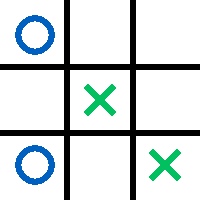
\includegraphics[scale=\scaling]{illustrations/board-example.pdf}
\end{center}\vspace{-\parskip}

Η σχετική λίστα θα αποτελείται από εννέα στοιχεία, σε κάθε ένα από τα οποία θα αποθηκεύεται το περιεχόμενο του αντίστοιχου τετραγώνου της τρίλιζας. Μια απεικόνιση της λίστας φαίνεται στο σχήμα~\ref{fig:board-representation-list.pdf} που ακολουθεί.
    
\marginnote[26pt]{Στην Python, όπως και σε πολλές άλλες γλώσσες, κάθε είδους αρίθμηση ξεκινά από το \pyinline{0}, όχι από το \pyinline{1}. Έτσι, το πρώτο στοιχείο αυτής της λίστας που αναπαριστά τον πίνακα του παιχνιδιού βρίσκεται στη θέση \pyinline{0} και το ένατο στη θέση \pyinline{8}.}
\marginnote{Γενικά, τα στοιχεία μιας λίστας μπορεί να είναι \emph{ο,τιδήποτε}, ακόμα και άλλες λίστες.}
\marginnote{Στη συγκεκριμένη περίπτωση, όλα τα στοιχεία της λίστας θα είναι αλφαριθμητικά και κάθε ένα από αυτά θα έχει τιμή είτε \pyinline{"X"}, είτε \pyinline{"O"}, είτε \pyinline{" "} (κενό).}
\vspace{-3pt}\begin{center}
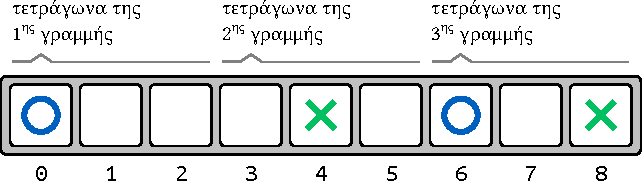
\includegraphics[scale=\scaling]{illustrations/board-representation-list.pdf}
\captionof{figure}{\label{fig:board-representation-list.pdf}Παράδειγμα αναπαράστασης ενός συγκεκριμένου στιγμιοτύπου του παιχνιδιού με τη χρήση \emph{λίστας}. Σε κάθε στοιχείο της λίστας αποθηκεύεται το περιεχόμενο ενός τετραγώνου της τρίλιζας. Η συγκεκριμένη αντιστοιχία μεταξύ τετραγώνων και στοιχείων της λίστας είναι απλά μία από τις πολλές που θα μπορούσαν να χρησιμοποιηθούν.}
\end{center}\vspace{-\parskip}

Η αναπαράσταση αυτή δεν είναι η μοναδική, υπάρχουν πολλές εναλλακτικές. Όμως δεν είναι εύκολο να γνωρίζουμε εκ των προτέρων ποια από τις πιθανές αναπαραστάσεις θ' αποδειχθεί βολικότερη. Ουσιαστικά, η επιλογή της κατάλληλης αναπαράστασης εξαρτάται από τον συγκεκριμένο τρόπο που το πρόγραμμά μας θα επεξεργάζεται τα δεδομένα. Εφόσον ακόμα δεν έχουμε γράψει το πρόγραμμα, μόνο η εμπειρία και η διαίσθηση μπορεί να μας καθοδηγήσει.

\section{Κάτι Να ``Μεταφράζει''}

% [review] Γιατί να ξεκινήσουμε από εδώ; Προς το παρόν στο μυαλό του αρχάριου δεν υπάρχει λόγος να φτιάξουμε κάτι τέτοιο. Άσε που για να το τεστάρει θα πρέπει να κατέβει 2 ενότητες παρακάτω. Το καταλαβαίνω ότι είναι μια ιδανική εισαγωγή γα τις θέσεις της λίστας, αλλά νοηματικά είναι πρώιμη η αναφορά στο υποπρόγραμμα. [update] Δεν το θεωρώ πρόβλημα, αλλά θα μπορούσαμε να το εντάξουμε στο Quick & Dirty, τη στιγμή που το χρειαζόμαστε.

\begin{question}
Εντάξει, επιλέξαμε την αναπαράσταση. Αλλά, όπως και να προχωρήσουμε, ο χρήστης θα πρέπει να βλέπει μια τρίλιζα για να παίζει, όχι εννέα τετράγωνα στη σειρά.
\end{question}

Ο τρόπος που το πρόγραμμα διαχειρίζεται ``εσωτερικά'' την αναπαράσταση της τρίλιζας δεν ενδιαφέρει το χρήστη. Στην οθόνη θα πρέπει να εμφανίζεται μια αναπαράσταση που να είναι γνώριμη στους παίκτες, δηλαδή ο κλασικός 3 $\times$ 3 πίνακας του παιχνιδιού. 

Θα ξεκινήσουμε λοιπόν κατασκευάζοντας ένα υποπρόγραμμα που δέχεται σαν παράμετρο την εσωτερική αναπαράσταση \pyinline{board} της τρίλιζας (εδώ πρόκειται για μια λίστα με εννέα στοιχεία) και την εμφανίζει στην οθόνη με τρόπο φιλικό προς το χρήστη.

% src/oxo.1.py: ορισμός της συνάρτησης print3χ3
\marginnote[18pt]{Μπορούμε ν' αναφερθούμε στα στοιχεία μιας λίστας με βάση τη \emph{θέση} τους σε αυτή. Η αρίθμηση των θέσεων ξεκινά από το \pyinline{0}. Έτσι, εδώ το πρώτο στοιχείο της λίστας \pyinline{board} είναι το \pyinline{board[0]}, το δεύτερο είναι το \pyinline{board[1]}, κ.ο.κ.}
\marginnote{Η παράμετρος \pyinline{trailing} καθορίζει αν θα εμφανιστεί μια κενή γραμμή μετά τον 3 $\times$ 3 πίνακα και έχει σαν \emph{προκαθορισμένη τιμή} την \pyinline{True}. Αυτό σημαίνει ότι υπάρχει η δυνατότητα να μην καθοριστεί η τιμή της παραμέτρου κατά την κλήση της συνάρτησης. Στην περίπτωση αυτή, η παράμετρος θα πάρει την προκαθορισμένη της τιμή.}
%\marginnote{\center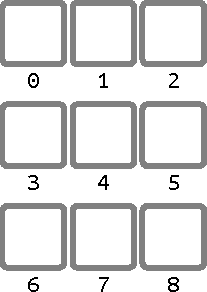
\includegraphics[scale=\scaling]{illustrations/board-representation-list-2d.pdf}%
%\captionof{figure}{\label{fig:board-representation-list-2d}%
%Η αντιστοιχία των εννέα στοιχείων της λίστας με τα εννέα τετράγωνα της τρίλιζας, όπως τα βλέπει ο χρήστης. Σε κάθε στοιχείο της λίστας, αριθμημένο από το \pyinline{0} μέχρι το \pyinline{8}, αποθηκεύεται το περιεχόμενο του αντίστοιχου τετραγώνου. Η αντιστοιχία αυτή είναι απλά μία από τις πολλές που θα μπορούσαν να χρησιμοποιηθούν.}}
\pysrc[firstline=1, lastline=12]{src/oxo.1.py}{}{}

% Το σχήμα~\ref{fig:board-representation-list-2d} δείχνει πως έχουμε αντιστοιχίσει τα εννέα στοιχεία της λίστας με τα τετράγωνα της τρίλιζας. 

Αυτή η αντιστοιχία ανάμεσα στα τετράγωνα και τις θέσεις της λίστας, όπως εξάλλου και η ίδια η αναπαράσταση με λίστα, αφορά μόνο εμάς ως προγραμματιστές και ο χρήστης ούτε τη γνωρίζει, ούτε τον αφορά. Όταν το πρόγραμμά μας θα καλεί την \pyinline{print3x3}, ο χρήστης θα βλέπει απλά στην οθόνη τα τετράγωνα της τρίλιζας. 

% Δεν είναι ανάγκη το πάνω αριστερά τετράγωνο να αντιστοιχεί στη θέση \pyinline{0}, ούτε το κεντρικό τετράγωνο στη θέση \pyinline{4}, κλπ. Αυτή είναι απλά μια από τις πολλές δυνατές αντιστοιχίες. 

\section{Quick and Dirty}

\begin{question}
Για αρχή, νομίζω ότι μπορώ να φτιάξω κάτι στα γρήγορα που να λειτουργεί. Δεν θα είναι τέλειο και στην πορεία θ' αλλάξω αρκετά πράγματα, όμως έτσι θα διαπιστώσω ποια σημεία παρουσιάζουν δυσκολίες.
\end{question}

\vspace{-12pt}
\subsection{Αρχικές τιμές}

Στο κύριο πρόγραμμα, η λίστα στην οποία θ' αποθηκεύουμε την τρέχουσα κατάσταση της τρίλιζας θα ονομάζεται \pyinline{board}. Αρχικά, πριν ξεκινήσει το παιχνίδι, η τρίλιζα θα περιέχει εννέα κενά τετράγωνα.

% src/oxo.1.py: αρχικοποίηση της board με 9 κενά στοιχεία
\marginnote[18pt]{Όταν ``πολλαπλασιάζουμε'' μια λίστα με τον τελεστή \pyinline{*} κατασκευάζουμε μια νέα λίστα που περιέχει πολλές φορές τα στοιχεία της αρχικής.}
\marginnote{Εδώ, η λίστα \pyinline{board} προκύπτει πολλαπλασιάζοντας  επί \pyinline{9} τη λίστα \pyinline{[" "]}, που αποτελείται από ένα στοιχείο.}
\pysrc[firstline=13, lastline=16]{src/oxo.1.py}{}{}

Όπως και στο \href{http://pythonies.mysch.gr/chapters/nim.pdf}{Παιχνίδι της Αφαίρεσης}, που ήταν επίσης παιχνίδι δύο παικτών, θα χρησιμοποιήσουμε μια μεταβλητή \pyinline{player}, η οποία σε κάθε γύρο θα παίρνει \emph{εναλλάξ} την τιμή \pyinline{"X"} ή \pyinline{"O"}, υποδεικνύοντας με αυτόν τον τρόπο ποιος έχει σειρά να παίξει σε κάθε γύρο.
Κατά σύμβαση, πρώτος παίζει ο παίκτης με τα X, οπότε πριν ξεκινήσει το παιχνίδι η \pyinline{player} θα πάρει την αντίστοιχη αρχική τιμή.

\clearpage
% src/oxo.1.py: αρχικοποίηση της player με το "Χ"
\marginnote[12pt]{\center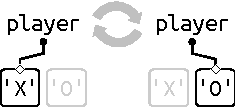
\includegraphics[scale=\scaling]{illustrations/player.pdf}
\captionof{figure}{Η τιμή της μεταβλητής \pyinline{player} θα εναλλάσσεται σε κάθε γύρο μεταξύ του \pyinline{"X"} και του \pyinline{"O"}, υποδεικνύοντας το σύμβολο του παίκτη που έχει σειρά να παίξει. Η αρχική της τιμή είναι το \pyinline{"Χ"}.}}
\pysrc[firstline=17, lastline=18]{src/oxo.1.py}{}{}

\subsection{Επανάληψη: η συνθήκη συνέχειας}

Ας περάσουμε τώρα στην επαναληπτική δομή. Κάθε κύκλος της επανάληψης αντιστοιχεί στη συμπλήρωση ενός τετραγώνου από κάποιο παίκτη. Για να ολοκληρωθεί το παιχνίδι και να \emph{τερματιστεί} η επανάληψη θα πρέπει είτε να συμπληρωθούν και τα εννέα τετράγωνα, είτε κάποιος από τους δύο παίκτες να κάνει τρίλιζα. Για να διατυπωθεί λοιπόν η συνθήκη της επανάληψης χρειάζεται το πρόγραμμα να καταμετρά το πλήθος των κενών τετραγώνων και να καταγράφει αν έχει γίνει τρίλιζα.

Για την καταμέτρηση των κενών τετραγώνων θα χρησιμοποιήσουμε τη μεταβλητή \pyinline{blank}. Όταν ξεκινά το παιχνίδι, όλα τα τετράγωνα είναι κενά.

% src/oxo.1.py: αρχικοποίηση της blank
\pysrc[firstline=19, lastline=20]{src/oxo.1.py}{}{}

Για να καταγράφει το πρόγραμμά μας αν έχει γίνει τρίλιζα ή όχι θα χρησιμοποιήσουμε μια λογική μεταβλητή \pyinline{inarow}. Γνωρίζουμε βέβαια πως όταν ξεκινά το παιχνίδι, κανείς από τους δύο παίκτες δεν έχει κάνει τρίλιζα κι έτσι η αρχική τιμή της \pyinline{inarow} θα πρέπει να είναι \pyinline{False}. 

% src/oxo.1.py: αρχικοποίηση της inarow
\pysrc[firstline=21, lastline=22]{src/oxo.1.py}{}{}

Είμαστε τώρα έτοιμοι να διατυπώσουμε τη συνθήκη της επανάληψης: για να \emph{συνεχιστεί} η επανάληψη θα πρέπει να απομένει τουλάχιστον ένα κενό τετράγωνο και ταυτόχρονα κανένας από τους δύο παίκτες να μην έχει κάνει τρίλιζα. 

% src/oxo.1.py: συνθήκη συνέχειας της while
%\marginnote[18pt]{Αντί για τη μεταβλητή \pyinline{blank}, θα μπορούσαμε στη θέση της να γράφαμε \pyinline{board.count(" ")}, η οποία επιστρέφει το πλήθος των κενών (\pyinline{" "}) στη λίστα \pyinline{board}. Όμως στην \pyinline{blank}, το πλήθος των κενών είναι \emph{αποθηκευμένο}, ενώ η \pyinline{count} το υπολογίζει κάθε φορά εξαρχής.}
\pysrc[firstline=23, lastline=25]{src/oxo.1.py}{}{}

\subsection{Επανάληψη: επιλογή κίνησης από τον παίκτη}

Μέσα στην επανάληψη, στην αρχή κάθε νέου κύκλου, το πρόγραμμα θα εμφανίζει τον πίνακα της τρίλιζας στον παίκτη που έχει σειρά να παίξει και θα τον ρωτάει σε ποιο τετράγωνο επιθυμεί να παίξει. 

%\begin{pyplain}
%    # εμφάνιση πίνακα τρίλιζας
%    print3x3(board)
%    # επιλογή θέσης από τον παίκτη
%    print(player, "διάλεξε τετράγωνο:", end=" ")
%    position = int(input())
%\end{pyplain}

Εδώ υπάρχει ένα πολύ λεπτό σημείο. Έστω ότι ζητάμε από το χρήστη να προσδιορίσει μ' έναν ακέραιο αριθμό το τετράγωνο στο οποίο θα παίξει. Υπονοείται λοιπόν ότι υπάρχει μια \emph{αρίθμηση} των τετραγώνων της τρίλιζας, με βάση την οποία θα κάνει την επιλογή του ο παίκτης. Έχει μεγάλη σημασία ότι η αυτή η αρίθμηση των τετραγώνων αφορά την οπτική γωνία \emph{του παίκτη}, τον τρόπο με τον οποίο θα προσδιορίσει το τετράγωνο που τον ενδιαφέρει και \emph{δεν έχει απαραίτητα σχέση} με την εσωτερική αναπαράσταση της τρίλιζας. 

\marginnote[-18pt]{\center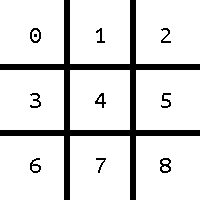
\includegraphics[scale=\scaling]{illustrations/board-user-simple.pdf}%
\captionof{figure}{Η αρίθμηση των τετραγώνων της τρίλιζας, από την σκοπιά του παίκτη. Με βάση αυτή την αρίθμηση επιλέγει ο παίκτης το τετράγωνο στο οποίο θα παίξει κάθε φορά. Θα μπορούσαμε να έχουμε επιλέξει μια διαφορετική αρίθμηση, αυτή όμως είναι βολική γιατί ταυτίζεται με την εσωτερική μας αναπαράσταση.\label{fig:board-user-simple}}}
Εμείς όμως προς το παρόν θα επιλέξουμε την απλούστερη δυνατή αρίθμηση, η οποία \emph{ταυτίζεται} με την αρίθμηση της εσωτερικής αναπαράστασης και φαίνεται στο σχήμα~\ref{fig:board-user-simple}. Ας έχουμε όμως υπόψη ότι αυτή η αρίθμηση είναι βολική για εμάς \emph{ως προγραμματιστές} και δεν είναι απαραίτητα η βολικότερη αρίθμηση \emph{για το χρήστη}.

Στον κώδικα που ακολουθεί, η \pyinline{print3x3} δεν χρησιμοποιείται μόνο για να εμφανιστεί ο πίνακας της τρίλιζας, αλλά επιστρατεύεται και μια δεύτερη φορά για να εμφανιστεί σε μορφή 3 $\times$ 3 πίνακα, σαν βοηθητικό υπόμνημα, η αρίθμηση με βάση την οποία θα επιλέξει τετράγωνο ο παίκτης.

% src/oxo.1.py: επιλογή τετραγώνου από τον παίκτη
\marginnote[0pt]{Η \pyinline{range} είναι μια \emph{ακολουθία} τιμών που ανήκουν σε ένα συγκεκριμένο \emph{διάστημα}. Όταν η \pyinline{range} καλείται με μια παράμετρο \pyinline{n}, τότε το διάστημα τιμών είναι από το \pyinline{0} μέχρι και το \pyinline{n-1}.}
\marginnote{Εδώ η \pyinline{range(9)} είναι η \emph{ακολουθία} των τιμών από το \pyinline{0} μέχρι και το \pyinline{8}, αντιστοιχεί δηλαδή στους αριθμούς των θέσεων της τρίλιζας.}
\pysrc[firstline=26, lastline=31]{src/oxo.1.py}{}{}

Όταν ο χρήστης επιλέξει αριθμό τετραγώνου, το πρόγραμμα θα συμπληρώνει την αναπαράσταση του πίνακα της τρίλιζας με το σύμβολο του παίκτη, ενώ παράλληλα θα μειώνει το πλήθος των κενών τετραγώνων.

% src/oxo.1.py: πραγματοποίηση κίνησης
\marginnote[12pt]{Χρησιμοποιώντας μια εντολή όπως η \pyinline{board[position] = player} \emph{τροποποιείται} το στοιχείο της λίστας \pyinline{board} που βρίσκεται στη θέση \pyinline{position}, το οποίο αντιστοιχεί πλέον σε μια νέα τιμή, την \pyinline{player}. Είναι ένα βασικό χαρακτηριστικό των λιστών ότι τα στοιχεία τους μπορούν να τροποποιηθούν.}
\marginnote{Η εντολή \pyinline{blank -= 1} μειώνει την τιμή της μεταβλητής \pyinline{blank} κατά μία μονάδα. Είναι ισοδύναμη με την εντολή \pyinline{blank = blank - 1}. Ανάλογες μορφές μεταβολής μιας μεταβλητής είναι διαθέσιμες για την αύξηση, τον πολλαπλασιασμό και γενικότερα όλες τις αριθμητικές πράξεις.}
\pysrc[firstline=32, lastline=37]{src/oxo.1.py}{}{}

\subsection{Επανάληψη: έλεγχος για τρίλιζα}

Μετά την κίνηση του παίκτη, το πρόγραμμά μας θα πρέπει να ελέγχει μήπως έγινε τρίλιζα. Προς το παρόν, θα υλοποιήσουμε αυτόν τον έλεγχο με τον πιο απλό τρόπο που μπορούμε να σκεφτούμε, εξετάζοντας όλες τις πιθανές τριάδες τετραγώνων. Στη συνέχεια θα έχουμε την ευκαιρία να διαπιστώσουμε αν υπάρχουν περιθώρια βελτίωσης.

% src/oxo.1.py: έλεγχος για τρίλιζα
\pysrc[firstline=38, lastline=46]{src/oxo.1.py}{}{continued}
\clearpage
\marginnote[18pt]{Μέχρι στιγμής έχουμε δει πως οι συγκριτικοί τελεστές χρησιμοποιούνται για να συγκρίνουν δύο τιμές μεταξύ τους. Στην Python μπορούν να χρησιμοποιηθούν για να συγκριθούν \emph{πολλές} τιμές μεταξύ τους, όπως σε αυτό το παράδειγμα με τον τελεστή \pyinline{==}. Αυτό είναι ένα χαρακτηριστικό που δεν το συναντάμε συχνά σε άλλες γλώσσες προγραμματισμού, με τους αντίστοιχους συγκριτικούς τελεστές.}
\pysrc[firstline=47, lastline=56]{src/oxo.1.py}{}{}

Κάθε μία από τις οκτώ περιπτώσεις σε αυτή τη δομή επιλογής αντιστοιχεί σε έναν από τους οκτώ διαφορετικούς τρόπους να γίνει τρίλιζα. Και στις οκτώ περιπτώσεις εκτελείται η ίδια εντολή: η μεταβλητή \pyinline{inarow} παίρνει την τιμή \pyinline{True}, για να καταγραφεί πλέον από το πρόγραμμα ότι έχει γίνει τρίλιζα (εναλλακτικά, θα μπορούσε να χρησιμοποιηθεί μια \emph{σύζευξη} των οκτώ επιμέρους συνθηκών). Παρατηρήστε ότι στη δομή επιλογής δεν υπάρχει \pyinline{else} επειδή δε χρειάζεται να εκτελεστεί κάποια εντολή σε περίπτωση που δε γίνει τρίλιζα.

\vspace{-6pt}
\subsection{Επανάληψη: εναλλαγή παίκτη}

Μέσα στην επανάληψη, απομένει μόνο να εναλλάσσουμε την τιμή της μεταβλητής \pyinline{player}.

% src/oxo.1.py: εναλλαγή παίκτη
\pysrc[firstline=57, lastline=61]{src/oxo.1.py}{}{}

\vspace{-6pt}
\subsection{Ανακοίνωση αποτελέσματος}

Όταν η επανάληψη τερματιστεί, το παιχνίδι θα έχει τελειώσει και το πρόγραμμα θα πρέπει να εμφανίσει στους παίκτες ποιο ήταν το αποτέλεσμα. Υπάρχουν δύο πιθανοί λόγοι για να τελειώσει το παιχνίδι: να έχει συμπληρωθεί ο πίνακας του παιχνιδιού ή να έχει γίνει τρίλιζα (χωρίς το ένα να αποκλείει το άλλο). Αν έχει γίνει τρίλιζα, θα πρέπει να εμφανίζεται κατάλληλο μήνυμα, διαφορετικά θα πρέπει να εμφανίζεται μήνυμα ότι το παιχνίδι έληξε ισόπαλο.

% src/oxo.1.py: εμφάνιση αποτελέσματος
\pysrc[firstline=62, lastline=68]{src/oxo.1.py}{}{οχο}

Είναι \emph{υποχρεωτικό} το πρόγραμμα να ελέγχει την τιμή της \pyinline{inarow} και όχι της \pyinline{blank} για να διαπιστώσει το αποτέλεσμα του παιχνιδιού. Η τιμή της \pyinline{blank} \emph{δεν} μπορεί να μας οδηγήσει σε ασφαλή συμπεράσματα, γιατί όταν έχει την τιμή \pyinline{0} μετά το τέλος του παιχνιδιού, δεν ξέρουμε με βεβαιότητα αν το παιχνίδι έληξε ισόπαλο ή αν η τελευταία κίνηση οδήγησε σε τρίλιζα.

\section{Συμμάζεμα}

\begin{question}
Ξέρω ότι μπορώ να ``σπάσω'' το πρόγραμμά μου σε μικρότερα τμήματα, υλοποιώντας τις επιμέρους λειτουργίες του προγράμματος ως ξεχωριστά υποπρογράμματα. Από που να ξεκινήσω;
\end{question}

% Φανταστείτε ότι εξηγείτε το πρόγραμμά σας σε κάποια φίλη σας. Αν της δείξετε μια ομάδα εντολών και της πείτε: ``να, με \emph{αυτές} εδώ τις εντολές, το πρόγραμμα κάνει μια συγκεκριμένη δουλειά'' τότε πιθανότατα έχετε εντοπίσει μια λειτουργία του προγράμματος που θα μπορούσε να υλοποιηθεί ως ξεχωριστό υποπρόγραμμα και να περιέχει λίγο-πολύ αυτές τις εντολές.

Είναι σημαντικό να διακρίνουμε (σε οποιοδήποτε πρόγραμμα) τις ομάδες εντολών που λειτουργούν ως ενιαίο σύνολο και υλοποιούν μια συγκεκριμένη λειτουργία. Αυτά τα τμήματα του προγράμματος θα αποτελέσουν τη βάση για την κατασκευή των επιμέρους υποπρογραμμάτων.

Ο τρόπος με τον οποίο μπορούμε να διαιρέσουμε ένα ενιαίο πρόγραμμα σε επιμέρους τμήματα με βάση τη λειτουργία τους δεν είναι μοναδικός. Στην πραγματικότητα υπάρχουν πολλές εναλλακτικές. Επίσης, οι εμπειρότεροι προγραμματιστές συνήθως \emph{σχεδιάζουν εκ των προτέρων} τα προγράμματά τους και τα υποπρογράμματα από τα οποία αποτελούνται, χωρίς αυτό να σημαίνει ότι στη συνέχεια, καθώς υλοποιούν το πρόγραμμά τους, δεν μπορούν να αναθεωρήσουν ή να εκλεπτύνουν τον αρχικό τους σχεδιασμό.

\subsection{Αλληλεπίδραση με το χρήστη}

Διατρέχοντας το πρόγραμμα που έχουμε αναπτύξει μέχρι στιγμής, εντοπίζουμε μέσα στην επαναληπτική δομή μια ομάδα εντολών που αναλαμβάνει την αλληλεπίδραση με τον παίκτη: εμφανίζει τα τετράγωνα της τρίλιζας και ρωτά τον παίκτη σε ποιο τετράγωνο επιθυμεί να παίξει.

% src/oxo.1.py: προέλευση της readPosition
\pysrc[firstline=26, lastline=31, linenos=false]{src/oxo.1.py}{plain}{}

Αυτή η ομάδα εντολών θ' αποτελέσει τη βάση για τη συνάρτηση \pyinline{readPosition}, η οποία δέχεται σαν παραμέτρους τον παίκτη \pyinline{player} που έχει σειρά να παίξει και την αναπαράσταση \pyinline{board} της τρίλιζας και επιστρέφει τη θέση που επέλεξε ο παίκτης για την επόμενη κίνησή του.

\clearpage
% src/oxo.2.py: ορισμός της readPosition
\marginnote[18pt]{Σε αυτή, αλλά και σε όλες τις συναρτήσεις που ακολουθούν, ονομάσαμε \pyinline{player} την παράμετρο που αντιστοιχεί στο σύμβολο του παίκτη και \pyinline{board} την παράμετρο που αντιστοιχεί στην αναπαράσταση της τρίλιζας. Χρησιμοποιήσαμε δηλαδή τα ίδια ονόματα που χρησιμοποιούνται και στο κύριο πρόγραμμα. Αυτό δεν είναι υποχρεωτικό, θα μπορούσαμε να χρησιμοποιήσουμε άλλα ονόματα για τις παραμέτρους, απλά θεωρούμε ότι έτσι το πρόγραμμα είναι πιο κατανοητό. Πρέπει όμως να γίνει σαφές ότι \emph{δεν πρόκειται για τις ίδιες μεταβλητές}: η \pyinline{player} και η \pyinline{board} του κύριου προγράμματος δεν ταυτίζονται με τις \emph{τοπικές} \pyinline{player} και \pyinline{board} μέσα σε μια συνάρτηση. Μάλιστα οι τοπικές μεταβλητές των συναρτήσεων δημιουργούνται μόνο όταν καλείται η συνάρτηση και παύουν να υφίστανται όταν ολοκληρωθεί η εκτέλεση των εντολών της.}
\pysrc[firstline=13, lastline=27]{src/oxo.2.py}{}{}

\subsection{Πραγματοποίηση κίνησης στο επιλεγμένο τετράγωνο}

Αμέσως μετά τις εντολές που ζητούν από τον παίκτη να επιλέξει το τετράγωνο στο οποίο θα παίξει, υπάρχει μια ομάδα εντολών που πραγματοποιούν την κίνηση του παίκτη.

% src/oxo.1.py: προέλευση της play
\pysrc[firstline=31, lastline=34, linenos=false]{src/oxo.1.py}{plain}{}

Αυτή η ομάδα εντολών θ' αποτελέσει τη βάση για τη συνάρτηση \pyinline{play}, η οποία δέχεται σαν παραμέτρους τον παίκτη \pyinline{player} που επέλεξε θέση, την αναπαράσταση \pyinline{board} της τρίλιζας και τη θέση που επέλεξε ο παίκτης και πραγματοποιεί την κίνησή του.

% src/oxo.2.py: ορισμός της play
\pysrc[firstline=28, lastline=38]{src/oxo.2.py}{}{}

\marginnote[-210pt]{\center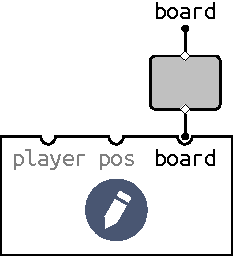
\includegraphics[scale=\scaling]{illustrations/function-play-call.pdf}%
\captionof{figure}{\label{fig:function-play-call}%
Όταν κληθεί η συνάρτηση \pyinline{play} από το κύριο πρόγραμμα, θα χρησιμοποιηθεί σαν παράμετρος η λίστα \pyinline{board} του κύριου προγράμματος. Η τοπική μεταβλητή \pyinline{board} της συνάρτησης \pyinline{play} και η \pyinline{board} του κύριου προγράμματος είναι δύο διαφορετικές μεταβλητές. Ωστόσο, είναι στην πραγματικότητα δύο διαφορετικά ονόματα για το ίδιο πράγμα: τη λίστα που αποτελεί την αναπαράσταση της τρίλιζας. Έτσι, οποιαδήποτε τροποποίηση γίνει εντός της συνάρτησης στα στοιχεία της λίστας \pyinline{board}, αφορά ουσιαστικά και τη λίστα \pyinline{board} του κύριου προγράμματος.%
}}
Η συνάρτηση \pyinline{play} δεν επιστρέφει κάποια τιμή, όμως \emph{μεταβάλλει την αναπαράσταση της τρίλιζας} (σχήμα~\ref{fig:function-play-call}).

% [comment][important] Συμπληρωματικές εξηγήσεις τόσο στο κείμενο, όσο και στα πλαινά σχόλια για την python.

\subsection{Έλεγχος για τρίλιζα}

Μια άλλη ομάδα εντολών που αποτελούν ενιαίο σύνολο απαρτίζεται από τη  δομή επιλογής που ελέγχει τις πιθανές τριάδες τετραγώνων για να διαπιστωθεί αν ο παίκτης που έπαιξε έκανε τρίλιζα.

% src/oxo.1.py: προέλευση της check
\pysrc[firstline=38, lastline=44, linenos=false]{src/oxo.1.py}{plain}{}
\begin{pyplain}
    |...|
\end{pyplain}
\pysrc[firstline=54, lastline=56, linenos=false]{src/oxo.1.py}{plain}{}

Αυτή η ομάδα εντολών θ' αποτελέσει τη βάση για τη συνάρτηση \pyinline{check}, η οποία δέχεται σαν παραμέτρους τον παίκτη \pyinline{player} που έχει σειρά να παίξει και την αναπαράσταση \pyinline{board} της τρίλιζας κι επιστρέφει \pyinline{True} ή \pyinline{False} ανάλογα αν ο παίκτης έκανε τρίλιζα ή όχι.

% src/oxo.2.py: ορισμός της check
\pysrc[firstline=39, lastline=65]{src/oxo.2.py}{}{}

\subsection{Εναλλαγή παίκτη}

Τέλος, οι εντολές που φροντίζουν για την εναλλαγή του παίκτη στο τέλος κάθε κύκλου της επανάληψης αποτελούν επίσης ένα ενιαίο σύνολο εντολών.

% src/oxo.1.py: προέλευση της next
\pysrc[firstline=57, lastline=61, linenos=false]{src/oxo.1.py}{plain}{}

Αυτή η ομάδα εντολών θ' αποτελέσει τη βάση για τη συνάρτηση \pyinline{next}, η οποία δέχεται σαν παράμετρο έναν παίκτη \pyinline{player} και επιστρέφει τον παίκτη που έχει σειρά να παίξει μετά από αυτόν.

% src/oxo.2.py: ορισμός της next
\pysrc[firstline=66, lastline=74]{src/oxo.2.py}{}{}

% [comment][important] Εδώ έχει αξία να σημειώσουμε ότι η next δεν μεταβάλλει (και δεν μπορεί να μεταβάλλει, χωρίς χρήση της global) την player του κύριου προγράμματος. [update] Έχουν φτιαχτεί σχετικά σχήματα. Όμως το (διόλου ευκαταφρόνητο) πρόβλημα είναι ότι υπάρχουν κι άλλα σημεία (κι εδώ και σε παλιότερα παραδείγματα) όπου πρέπει να εξηγηθεί το ίδιο πράγμα. Πχ. το ίδιο συμβαίνει και με την position στην readPosition. Γιατί πρέπει να επιστρέφει τιμή; Δεν αρκεί η position = int(input()); Δεν πρέπει να εξηγηθούν αυτά;

\subsection{Το κύριο πρόγραμμα}

Τώρα, το κύριο πρόγραμμα μπορεί να καλεί αυτές τις συναρτήσεις. Στο σημείο όπου το πρόγραμμα αλληλεπιδρά με το χρήστη για να τον ρωτήσει σε ποιο τετράγωνο επιθυμεί να παίξει, καλείται η συνάρτηση \pyinline{readPosition}. Στο σημείο όπου πραγματοποιείται η κίνηση του παίκτη, καλείται η \pyinline{play}. Στο σημείο όπου ελέγχεται αν η κίνηση του παίκτη οδηγεί σε τρίλιζα, καλείται η \pyinline{check}. Τέλος, αμέσως μετά, στο σημείο όπου εναλλάσσεται ο παίκτης που έχει σειρά να παίξει, καλείται η \pyinline{next}.

% src/oxo.2.py: κύριο πρόγραμμα (με αλλαγές)
\pysrc[firstline=85, lastline=87]{src/oxo.2.py}{plain}{continued}
\pysrc[firstline=88, lastline=91]{src/oxo.2.py}{}{continued}
\pysrc[firstline=92, lastline=93]{src/oxo.2.py}{plain}{continued}
\pysrc[firstline=94, lastline=97]{src/oxo.2.py}{}{}

Τώρα πλέον το μέγεθος του κύριου προγράμματος έχει μειωθεί δραματικά, ενώ έχει βελτιωθεί κατά πολύ η αναγνωσιμότητά του.

\section{Το Ζήτημα του Νικητή}

\begin{question}
Θα ήθελα το πρόγραμμα ν' ανακοινώνει ποιος παίκτης κέρδισε.
\end{question}

Σε περίπτωση που γίνει τρίλιζα, το πρόγραμμα εμφανίζει το μήνυμα \pyinline{"Τρίλιζα!"}, χωρίς όμως ν' ανακοινώνει ποιος από τους δύο παίκτες κέρδισε. Προφανώς, πρόκειται για τον παίκτη που έπαιξε τελευταίος κι έτσι μια βιαστική λύση θα ήταν να εμφανίσουμε το νικητή τροποποιώντας τις εντολές εμφανίζουν το αποτέλεσμα ως εξής:

\begin{pyplain}
# εμφάνιση αποτελέσματος
if inarow:
\end{pyplain}
\begin{pynew}
    print("Τρίλιζα! Κέρδισε ο", player)
\end{pynew}
\begin{pyplain}
else:
    print("Ισοπαλία.")
\end{pyplain}

Εδώ όμως υπάρχει πρόβλημα. Η μεταβλητή \pyinline{player} εναλλάσσεται \emph{στο τέλος} κάθε κύκλου της επανάληψης, ακόμα κι όταν κάποιος παίκτης κάνει τρίλιζα. Έτσι, μετά τον τερματισμό της επανάληψης, η \pyinline{player} δεν αντιστοιχεί στον παίκτη που έπαιξε τελευταίος (και κέρδισε), αλλά στον επόμενο (που είναι ο ηττημένος). Επομένως, αν το πρόγραμμα απλά εμφανίσει την τιμή της \pyinline{player}, θα εμφανίσει τον παίκτη που \emph{έχασε}, όχι εκείνον που έκανε τρίλιζα. 

Για να διορθώσουμε αυτή την συμπεριφορά θα υιοθετήσουμε μια λύση που απαιτεί τις λιγότερες αλλαγές στο πρόγραμμά μας: ο νικητής του παιχνιδιού είναι ο παίκτης που θα έπαιζε μετά τον ηττημένο.

% src/oxo.2.py: εμφάνιση αποτελέσματος (με νικητή)
\pysrc[firstline=100, lastline=101]{src/oxo.2.py}{plain}{continued}
\pysrc[firstline=102, lastline=102]{src/oxo.2.py}{}{continued}
\pysrc[firstline=103, lastline=104]{src/oxo.2.py}{plain}{oxo}

\section{Το Ζήτημα του Ελέγχου}

\begin{question}
Όταν ο χρήστης επιλέγει το τετράγωνο στο οποίο θα παίξει, το πρόγραμμα του επιτρέπει να πληκτρολογήσει οποιονδήποτε αριθμό, χωρίς κανέναν έλεγχο αν αυτός βρίσκεται μεταξύ \pyinline{0} και \pyinline{8}. Δεν ελέγχεται καν αν το τετράγωνο που επιλέγει ο χρήστης είναι κατειλημμένο.
\end{question}

Η επιλογή τετραγώνου από τον παίκτη πραγματοποιείται μέσω της συνάρτησης \pyinline{readPosition}. Αυτή θα πρέπει τώρα να \emph{επεκταθεί}, έτσι ώστε η τιμή που πληκτρολογεί ο παίκτης να ελέγχεται και, σε περίπτωση που δεν είναι έγκυρη, να ζητείται νέα τιμή.

Μέσα στη \pyinline{readPosition}, οι εντολές που ζητούν από τον παίκτη να επιλέξει το τετράγωνο στο οποίο θα παίξει θα τοποθετηθούν πλέον μέσα σε μια επαναληπτική δομή. Έτσι, ο παίκτης θα ``εγκλωβίζεται'' σε έναν κύκλο από τον οποίο βγαίνει μόνο όταν πληκτρολογήσει μια έγκυρη τιμή. Αν ο παίκτης επιλέξει θέση που δεν είναι ανάμεσα στο \pyinline{0} και το \pyinline{8} ή επιλέξει κατειλημμένη θέση τότε εμφανίζεται μήνυμα λάθους και η ανάγνωση τιμής επαναλαμβάνεται.

% [comment] ιδιαίτερα λεπτό σημείο η διάκριση ανάμεσα στην τιμή που δίνει ο παίκτης και την αντίστοιχη θέση στη λίστα. Οι έλεγχοι αφορούν και την τιμή και τη θέση. Τα μηνύματα αφορούν μόνο την τιμή. [update] Αυτή την στιγμή *δεν* διακρίνουμε ανάμεσα στα δύο. 

% src/oxo.3.py: τροποποίηση της readPosition για να κάνει έλεγχο
\pysrc[firstline=20, lastline=22]{src/oxo.3.py}{plain}{continued}
\pysrc[firstline=23, lastline=24]{src/oxo.3.py}{}{continued}
\pysrc[firstline=25, lastline=27]{src/oxo.3.py}{plain}{continued}
\pysrc[firstline=28, lastline=35]{src/oxo.3.py}{}{continued}
\pysrc[firstline=36, lastline=37]{src/oxo.3.py}{plain}{oxo}

Στο κύριο πρόγραμμα δεν απαιτείται καμία αλλαγή. Εκεί εξακολουθεί να καλείται η \pyinline{readPosition}, από την οποία προκύπτει η θέση στην οποία θα τοποθετήσει το σύμβολό του ο παίκτης. Όμως τώρα η τιμή που θα επιστρέψει η τροποποιημένη \pyinline{readPosition} θα είναι σίγουρα έγκυρη.

\section{Το Ζήτημα της Τρίλιζας}

\begin{question}
Η συνάρτηση \pyinline{check} μου κάθεται στο λαιμό. Δεν γίνεται να υλοποιήσουμε τον έλεγχο αν έχει γίνει τρίλιζα με πιο κομψό, συμπαγή τρόπο;
\end{question}

Αν μελετήσουμε τη μεγάλη \pyinline{if} που βρίσκεται μέσα στη συνάρτηση \pyinline{check} και ελέγχει τους οκτώ διαφορετικούς τρόπους να γίνει τρίλιζα, θα παρατηρήσουμε ότι οι οκτώ συνθήκες που ελέγχονται είναι ουσιαστικά ίδιες μεταξύ τους. Κάθε συνθήκη εξετάζει μια τριάδα θέσεων και το μόνο που αλλάζει από περίπτωση σε περίπτωση είναι \emph{οι αριθμοί των τριών θέσεων που ελέγχονται}.

Ας καταγράψουμε λοιπόν σε μια κατάλληλη δομή τις διαφορετικές τριάδες θέσεων που εξετάζονται.

% src/oxo.4.py: τριάδες τετραγώνων που σχηματίζουν τρίλιζα
\marginnote[-96pt]{Μια δομή δεδομένων που μοιάζει πολύ με τις λίστες είναι οι \emph{πλειάδες} (tuples). Τα περιεχόμενα των πλειάδων περικλείονται σε παρενθέσεις και, σε αντίθεση με τις λίστες, \emph{δεν} μπορούν να μεταβληθούν. Η πρόσβαση στα στοιχεία των πλειάδων γίνεται ακριβώς με τον ίδιο τρόπο όπως και στις λίστες.}
\marginnote{Εδώ θέλουμε ν' αποτυπώσουμε τις διαφορετικές τριάδες θέσεων που σχηματίζουν τρίλιζες. Επειδή αυτές οι τιμές δεν πρόκειται ν' αλλάξουν, %κατά τη διάρκεια εκτέλεσης του προγράμματος, 
χρησιμοποιείται για την αποθήκευσή τους μια πλειάδα, η \pyinline{triples}.}
\marginnote{Η \pyinline{triples} είναι μια πλειάδα που περιέχει άλλες πλειάδες. Συγκεκριμένα, περιέχει τριάδες με τους αριθμούς των θέσεων που σχηματίζουν τρίλιζες.}
\pysrc[firstline=73, lastline=77, linenos=False]{src/oxo.4.py}{plain}{}

Αυτό το τμήμα κώδικα που ορίζει την \pyinline{triples}, μπορούμε να το εισάγουμε στη συνάρτηση \pyinline{check}. Στην περίπτωση αυτή, θα πρόκειται για μια \emph{τοπική} μεταβλητή της συνάρτησης. Θα δημιουργείται εκ νέου κάθε φορά που θα καλείται η \pyinline{check} και θα παύει να υφίσταται όταν τελειώνει η εκτέλεσή της. 
% Για το λόγο αυτό, το κύριο πρόγραμμα και οι υπόλοιπες συναρτήσεις δεν θα μπορούν να αναφερθούν στην \pyinline{triples}.

Εμείς όμως θα προτιμήσουμε να ορίσουμε την \pyinline{triples} \emph{στην αρχή του κύριου προγράμματος}. Θα είναι έτσι μια \emph{καθολική} μεταβλητή. Θα μπορούν να αναφερθούν σε αυτήν (αλλά όχι να την  τροποποιήσουν) όλες οι συναρτήσεις, συμπεριλαμβανομένης και της \pyinline{check} φυσικά.

% [comment] Πως μπορούμε να εξηγήσουμε γιατί αυτό το θεωρούμε προτιμότερο;

Διατρέχοντας τις οκτώ τριάδες που περιέχει η \pyinline{triples}, μπορούμε να ελέγξουμε \emph{επαναληπτικά}, για κάθε μια από αυτές, αν είναι πλήρως συμπληρωμένη από έναν συγκεκριμένο παίκτη. Η συνάρτηση \pyinline{check} μπορεί πλέον να ξαναγραφτεί με πιο συμπαγή τρόπο.

% src/oxo.4.py: τροποποίηση της check με πλειάδες
\marginnote[18pt]{Η εντολή \pyinline{for} είναι μια εντολή επανάληψης που διατρέχει τα στοιχεία μιας ακολουθίας τιμών, όπως μια λίστα ή μια πλειάδα, με τη σειρά με την οποία αυτά εμφανίζονται στην ακολουθία. Σε κάθε επανάληψη, η τιμή του επόμενου στοιχείου της ακολουθίας ανατίθεται στη \emph{μεταβλητή απαρίθμησης} που χρησιμοποιούμε στη \pyinline{for}.}
\marginnote{Εδώ η \pyinline{for} χρησιμοποιείται για να διατρεχθούν όλες οι τριάδες της πλειάδας \pyinline{triples}.}
\marginnote{Με την εντολή \pyinline{p1, p2, p3 = triple} οι τρεις τιμές που βρίσκονται αποθηκευμένες στην πλειάδα \pyinline{triple} αποδίδονται στις μεταβλητές \pyinline{p1}, \pyinline{p2} και \pyinline{p3} αντίστοιχα.}
\marginnote{Αυτό ονομάζεται \emph{ξεπακετάρισμα} της πλειάδας (tuple unpacking) και είναι ουσιαστικά ο μηχανισμός που χρησιμοποιείται και για την επιστροφή πολλαπλών τιμών από συναρτήσεις.}
\pysrc[firstline=49, lastline=54]{src/oxo.4.py}{plain}{continued}
\pysrc[firstline=55, lastline=63]{src/oxo.4.py}{}{οχο}

Αν και η συνάρτηση \pyinline{check} ουσιαστικά ξαναγράφτηκε από την αρχή, η \emph{λειτουργία} της παρέμεινε η ίδια: ελέγχει αν έχει γίνει τρίλιζα. Γι' αυτό και δεν απαιτείται καμία τροποποίηση στο κύριο πρόγραμμα. Αυτό που άλλαξε είναι η \emph{υλοποίηση} αυτής της λειτουργίας, δηλαδή ο τρόπος με τον οποίο ελέγχεται αν έχει γίνει τρίλιζα. 

\section{Κάτι Για Παρέα}

\begin{question}
Στην αρχή είπαμε ότι θα φτιάξουμε ένα πρόγραμμα που θα παίζει τρίλιζα. Προς το παρόν και οι δύο παίκτες που συμμετέχουν στο παιχνίδι είναι άνθρωποι.
\end{question}

Θα κάνουμε τις απαραίτητες επεκτάσεις, ώστε το πρόγραμμα ν' αναλάβει το ρόλο ενός από τους δύο παίκτες. Δεν είναι ανάγκη να προσπαθήσουμε εξαρχής να κάνουμε το πρόγραμμα να παίζει έξυπνα. Με αυτό θα ασχοληθούμε στο επόμενο βήμα· προς το παρόν, θα του επιτρέψουμε να ξεκινάει πρώτο και να επιλέγει σε κάθε γύρο μια τυχαία κίνηση.

Αφού οι κινήσεις του προγράμματος θα είναι τυχαίες, χρειάζεται να εισαγάγουμε, στην αρχή του προγράμματος, την κατάλληλη βιβλιοθήκη.

% src/oxo.5.py: import random
\pysrc[firstline=1, lastline=1]{src/oxo.5.py}{}{}

\subsection{Οι διαθέσιμες θέσεις}

Για να επιλέξει το πρόγραμμα σε ποια θέση θα παίξει, θα πρέπει πρώτα να υπολογίσει ποιες από τις εννέα θέσεις είναι διαθέσιμες. 

Αυτό μπορεί να γίνει με τον κώδικα που ακολουθεί, ο οποίος διατρέχει τις εννέα θέσεις της τρίλιζας και κατασκευάζει μια λίστα με τις θέσεις εκείνες που είναι διαθέσιμες.

\marginnote[18pt]{Η \pyinline{range} χρησιμοποιείται για να αναφερθούμε σε ένα \emph{διάστημα τιμών}. Η προαιρετική πρώτη παράμετρος ορίζει το αριστερό άκρο του διαστήματος. Αν παραληφθεί, το διάστημα ξεκινά από το \emph{μηδέν}. Η δεύτερη παράμετρος ορίζει το δεξί άκρο, το οποίο είναι ανοικτό (δηλαδή το διάστημα δεν περιλαμβάνει την τιμή που δίνεται σαν δεξί άκρο). Η προαιρετική τρίτη παράμετρος ορίζει το \emph{βήμα}, δηλαδή ανά πόσες τιμές του διαστήματος θα διατρέχονται.}
\marginnote{Η μέθοδος \pyinline{append()} εφαρμόζεται σε μια λίστα και προσθέτει ένα νέο στοιχείο στο τέλος της.}
\marginnote{Εδώ η \pyinline{append()} καλείται επαναληπτικά, κατασκευάζοντας στοιχείο προς στοιχείο τη λίστα με τις διαθέσιμες θέσεις.}
\begin{pyplain}
# η λίστα με τις διαθέσιμες θέσεις, αρχικά κενή
positions = []
# για κάθε θέση από 0 μέχρι και 8
for s in range(9):
    # αν η θέση s είναι διαθέσιμη
    if board[s] == " ":
        # προστίθεται στη λίστα διαθέσιμων θέσεων
        positions.append(s)
\end{pyplain}

Είναι συνηθισμένο να κατασκευάζουμε λίστες με αυτόν ακριβώς τον τρόπο, ξεκινώντας από μια κενή λίστα στην οποία προσθέτουμε σταδιακά τις τιμές που ικανοποιούν ένα συγκεκριμένο κριτήριο. Είναι τόσο συνηθισμένο αυτό το μοτίβο, που υπάρχει κι ένας εναλλακτικός, συνοπτικότερος τρόπος να δημιουργηθεί η ίδια λίστα:

\marginnote{Η \emph{συγκέντρωση λίστας} (list comprehension), είναι ένας συνοπτικός και εύληπτος τρόπος να δημιουργήσουμε μια λίστα περιγράφοντας τα στοιχεία της, από που αυτά προέρχονται και πως επιλέγονται.}
\marginnote{Εδώ συγκεντρώνουμε σε μια λίστα όλα τα στοιχεία \pyinline{s} που περιέχονται στο διάστημα μεταξύ \pyinline{0} και \pyinline{8} και έχουν το χαρακτηριστικό ότι το \pyinline{board[s]} έχει την τιμή \pyinline{" "} (κενό).}
\begin{pyplain}
# συγκέντρωση λίστας: λίστα με τις διαθέσιμες θέσεις s
positions = [s for s in range(9) if board[s] == " "]
\end{pyplain}

Ουσιαστικά εδώ \emph{περιγράφουμε} από τι αποτελείται η \pyinline{positions}, όπως θα κάναμε στα μαθηματικά: είναι μια λίστα από όλες τις θέσεις \pyinline{s}, μεταξύ \pyinline{0} και \pyinline{8}, για τις οποίες ισχύει ότι το \pyinline{board[s]} είναι κενό, δηλαδή η αντίστοιχη θέση της τρίλιζας είναι διαθέσιμη.

Τώρα μπορούμε να ορίσουμε τη συνάρτηση \pyinline{available}, η οποία δέχεται σαν παράμετρο την αναπαράσταση \pyinline{board} της τρίλιζας και επιστρέφει \emph{μια νέα λίστα} με τους αριθμούς των διαθέσιμων θέσεων.

% src/oxo.5.py: ορισμός της available
\pysrc[firstline=79, lastline=83]{src/oxo.5.py}{}{}

\subsection{Τυχαία επιλογή θέσης}

Έχοντας κατασκευάσει τη συνάρτηση \pyinline{available}, η οποία επιστρέφει μια λίστα με τις διαθέσιμες θέσεις, είναι εύκολο να προχωρήσουμε και στον ορισμό της συνάρτησης \pyinline{randomPosition}, η οποία δέχεται σαν παράμετρο την αναπαράσταση \pyinline{board} της τρίλιζας και επιστρέφει μια τυχαία επιλεγμένη διαθέσιμη θέση.

% src/oxo.5.py: ορισμός της randomPosition
\marginnote[18pt]{Η συνάρτηση \pyinline{choice()} της βιβλιοθήκης \pyinline{random} δέχεται σαν παράμετρο μια λίστα κι επιστρέφει ένα τυχαία επιλεγμένο στοιχείο της.}
\marginnote{Εδώ χρησιμοποιείται για την τυχαία επιλογή μιας θέσης, από τη λίστα των διαθέσιμων θέσεων.}
\pysrc[firstline=79, lastline=83]{src/oxo.5.py}{}{}

%\begin{pyplain}
%# υπολογισμός διαθέσιμων θέσεων
%positions = available(board)
%# τυχαία επιλογή μιας διαθέσιμης θέσης
%position = random.choice(positions)
%\end{pyplain}

%\begin{pyplain}
%possible = available(board)
%index = random.randint(0, len(possible)-1)
%position = possible[index]
%\end{pyplain}

\subsection{Επεκτάσεις στο κύριο πρόγραμμα}

Ως τώρα, έχουμε προσθέσει στο πρόγραμμα την απαραίτητη υποδομή ώστε να είναι δυνατή η επιλογή μιας τυχαίας θέσης. Ωστόσο, το κύριο πρόγραμμα εξακολουθεί να υλοποιεί ένα παιχνίδι δύο παικτών. Θα πρέπει λοιπόν να επεκτείνουμε το κύριο πρόγραμμα, ώστε ν' αναλαμβάνει πλέον το ρόλο ενός από τους δύο παίκτες. 

Θα χρησιμοποιήσουμε τη μεταβλητή \pyinline{computer}, της οποίας η τιμή θ’ αντιστοιχεί στο σύμβολο του παίκτη που θα παίζει αυτοματοποιημένα. Στην αρχή του παιχνιδιού η \pyinline{computer} θα παίρνει την τιμή \pyinline{"X"}, ώστε το πρόγραμμα να παίζει πρώτο.

% src/oxo.5.py: αρχικοποίηση της computer
\pysrc[firstline=95, lastline=96]{src/oxo.5.py}{}{}

\marginnote{\center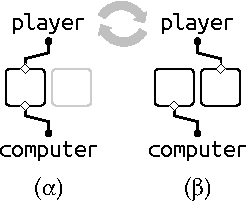
\includegraphics[scale=\scaling]{illustrations/player-computer.pdf}
\captionof{figure}{Επιλογή κίνησης, ανάλογα με τον παίκτη: (α) αν η \pyinline{computer} έχει ίδια τιμή με την \pyinline{player}, τότε είναι σειρά του προγράμματος να παίξει, ενώ (β) σε διαφορετική περίπτωση, έχει σειρά να παίξει ο χρήστης.}}
Θυμηθείτε ότι η μεταβλητή \pyinline{player} εναλλάσσεται σε κάθε γύρο μεταξύ των τιμών \pyinline{"X"} και \pyinline{"O"}, υποδεικνύοντας ποιος παίκτης έχει σειρά να παίξει στον επόμενο γύρο. Συκρίνοντας λοιπόν την \pyinline{player} με την \pyinline{computer} ελέγχουμε ουσιαστικά αν ο επόμενος παίκτης είναι ο άνθρωπος ή το πρόγραμμά μας.
% ώστε να καλέσουμε σε κάθε περίπτωση την ανάλογη συνάρτηση που θα μας επιστρέψει τη θέση που επιλέγει ο παίκτης για να παίξει.
Αν είναι σειρά του προγράμματος να παίξει, καλείται η \pyinline{randomPosition}, ενώ σε διαφορετική περίπτωση καλείται η \pyinline{readPosition}, ώστε να επιλέξει ο χρήστης τη θέση στην οποία επιθυμεί να παίξει.

% src/oxo.5.py: τροποποίηση του κύριου προγράμματος
% \pysrc[firstline=93, lastline=95]{src/oxo.5.py}{plain}{continued}
\pysrc[firstline=104, lastline=107]{src/oxo.5.py}{}{continued}
\pysrc[firstline=108, lastline=109]{src/oxo.5.py}{plain}{oxo}

\section{Κάτι ``Εξυπνότερο'' Για Παρέα}

\begin{question}
Ωραία, τώρα το πρόγραμμμα παίζει με τον παίκτη, αλλά οι κινήσεις του είναι αστείες. Παίζει τυχαία ακόμα κι όταν του δίνεται η ευκαιρία να κερδίσει. Παίζει τυχαία ακόμα κι όταν ο αντίπαλός του ετοιμάζεται να κάνει τρίλιζα. Θέλω να παίζει ``εξυπνότερα''.
\end{question}

Το λιγότερο που μπορούμε να κάνουμε είναι να επεκτείνουμε το πρόγραμμα έτσι ώστε να ελέγχει πότε ένας παίκτης έχει \emph{τη δυνατότητα} να κάνει τρίλιζα. Έτσι, όταν έχει την ευκαιρία, το πρόγραμμα θα μπορεί να κερδίζει ή, τουλάχιστον, να εμποδίζει τον αντίπαλό του.

Ένας παίκτης έχει τη δυνατότητα να κάνει τρίλιζα όταν υπάρχει τριάδα στην οποία \emph{οι δύο θέσεις} είναι ήδη κατειλημμένες από τον παίκτη και η τρίτη είναι κενή.

Η συνάρτηση \pyinline{check} που περιέχει \emph{ήδη} το πρόγραμμά μας ελέγχει κάτι παρεμφερές: αν υπάρχει τριάδα στην οποία \emph{και οι τρεις θέσεις} είναι ήδη κατειλημμένες από έναν παίκτη. 

Μπορούμε λοιπόν να βασιστούμε στον κώδικα της \pyinline{check}, κάνοντας τις κατάλληλες τροποποιήσεις, και να φτιάξουμε τη νέα συνάρτηση \pyinline{checkPartial}, η οποία δέχεται σαν παραμέτρους τον παίκτη \pyinline{player} που έχει σειρά να παίξει και την αναπαράσταση \pyinline{board} της τρίλιζας και ελέγχει αν ο παίκτης έχει τη δυνατότητα να κάνει τρίλιζα. Η συνάρτηση επιστρέφει τον αριθμό της θέσης στην οποία πρέπει να παίξει ο παίκτης \pyinline{player} για να κάνει τρίλιζα ή, αν δεν υπάρχει τέτοια θέση, την ειδική τιμή \pyinline{None}.

% [comment] Εδώ υπάρχουν *πολλοί* διαφορετικοί τρόποι υλοποίησης. Να δώσουμε ένα link με μερικές από τις εναλλακτικές.

% src/oxo.6.py: υλοποίηση της checkPartial
\marginnote[18pt]{Η χρήση των παρενθέσεων στις συνθήκες της \pyinline{if} δεν είναι υποχρεωτική. Είναι όμως ένας από τους πιθανούς τρόπους να υποδηλώσουμε ότι πρόκειται για ``μεγάλες'' γραμμές που συνεχίζονται και στην επόμενη γραμμή. Ένας άλλος τρόπος είναι η χρήση της καθέτου \textbackslash\ στο τέλος κάθε τέτοιας μεγάλης γραμμής.}
\pysrc[firstline=65, lastline=87]{src/oxo.6.py}{}{}

Η \pyinline{checkPartial}, όπως και η \pyinline{check}, διατρέχει τις τριάδες θέσεων που σχηματίζουν τρίλιζες. Όμως η \pyinline{checkPartial} ελέγχει, για κάθε τριάδα, αν είναι \emph{σχεδόν} συμπληρωμένη από έναν παίκτη και επιστρέφει τον αριθμό της θέσης που απομενει να συμπληρωθεί.

\subsection{Τυχαιότητα με Μέτρο}

Έχοντας στη διάθεσή μας την \pyinline{checkPartial}, μπορούμε να επεκτείνουμε την \pyinline{randomPosition} έτσι ώστε ο παίκτης με τα Χ να παίζει τυχαία μόνο όταν δεν έχει την ευκαιρία να νικήσει ή να εμποδίσει τον αντίπαλό του.

Επειδή αυτή η ευκαιρία παρουσιάζεται μετά τη δεύτερη κίνηση, η \pyinline{randomPosition} θα ξεκινά πλέον με τον κώδικα που ακολουθεί:

% src/oxo.6.py: τροποποίηση της randomPosition: πλήθος κινήσεων
\marginnote[18pt]{Η μέθοδος \pyinline{count} εφαρμόζεται σε μια λίστα. Δέχεται σαν παράμετρο μια τιμή και επιστρέφει το πλήθος των εμφανίσεων αυτής της τιμής στη λίστα.}
\marginnote{Εδώ η \pyinline{count} χρησιμοποιείται για να μετρήσουμε το πλήθος των \pyinline{"X"} στη λίστα \pyinline{board}, δηλαδή πόσες φορές έχει ήδη παίξει ο παίκτης με τα Χ.}

% \pysrc[firstline=99, lastline=104]{src/oxo.6.py}{plain}{continued}
\pysrc[firstline=108, lastline=109]{src/oxo.6.py}{}{}

Αν έχουν γίνει τουλάχιστον δύο κινήσεις, ελέγχεται αν υπάρχει θέση στην οποία μπορεί να παίξει ο παίκτης με τα X και να κάνει τρίλιζα. Αν υπάρχει, η \pyinline{randomPosition} επιστρέφει αυτή τη θέση, αντί μιας τυχαίας, επιτρέποντας στον παίκτη με τα Χ να κερδίσει.

% src/oxo.6.py: τροποποίηση της randomPosition: part I
\pysrc[firstline=110, lastline=115]{src/oxo.6.py}{}{}

Στη συνέχεια, ελέγχεται αν υπάρχει θέση στην οποία μπορεί να παίξει ο παίκτης με τα Ο και να κάνει τρίλιζα. Αν υπάρχει, επιστρέφεται αυτή η θέση, αντί μιας τυχαίας, επιτρέποντας στον παίκτη με τα Χ να εμποδίσει τον αντίπαλό του από το να κάνει τρίλιζα. 

% src/oxo.6.py: τροποποίηση της randomPosition: part II
\pysrc[firstline=116, lastline=119]{src/oxo.6.py}{}{continued}
\pysrc[firstline=120, lastline=121]{src/oxo.6.py}{plain}{oxo}

Τώρα η \pyinline{randomPosition} επιστρέφει μια τυχαία θέση μόνο αν δεν προκύψει αποτέλεσμα από την όλη διαδικασία που προηγείται.

%\marginnote[18pt]{Συλλογές όπως οι λίστες, οι πλειάδες και τα αλφαριθμητικά, μπορούν να \emph{τεμαχιστούν} (slicing). Με τον τεμαχισμό επιλέγεται ένα τμήμα μιας συλλογής, από το οποίο δημιουργείται μια νέα. Για να γίνει τεμαχισμός, πρέπει να προσδιοριστεί από ποια θέση θα ξεκινήσει, σε ποια θα σταματήσει και ανά πόσα στοιχεία θα επιλέγονται.}
%\marginnote[10pt]{Η έκφραση \pyinline{triple[1:]} είναι ένα παράδειγμα τεμαχισμού. Δημιουργεί μια νέα πλειάδα η οποία περιέχει τα στοιχεία της \pyinline{triple} από το δεύτερο (θέση \pyinline{1}) μέχρι και το τελευταίο. Γενικά, αν παραλειφθεί η θέση τερματισμού, τότε ο τεμαχισμός σταματά στο τέλος της λίστας, περιλαμβάνοντας και το τελευταίο στοιχείο.}
%\marginnote{Η έκφραση \pyinline{triple[::2]} δημιουργεί μια νέα πλειάδα η οποία περιέχει \emph{ανά δύο} τα στοιχεία της \pyinline{triple} από το πρώτο μέχρι και το τελευταίο. Γενικά, όταν το βήμα τεμαχισμού δεν προσδιορίζεται, θεωρείται ότι είναι το \pyinline{1}.}
%\marginnote{Η έκφραση \pyinline{triple[:2]} δημιουργεί μια νέα πλειάδα η οποία περιέχει τα στοιχεία της \pyinline{triple} από το πρώτο μέχρι το τρίτο (θέση \pyinline{2}), χωρίς να το περιλαμβάνει. Γενικά, ο τεμαχισμός σταματά \emph{πριν} το στοιχείο που βρίσκεται στη θέση τερματισμού. Αν παραλειφθεί η θέση εκκίνησης, τότε ο τεμαχισμός ξεκινά από την αρχή της λίστας. }
%\pysrc[firstline=60, lastline=61]{src/oxo.6.py}{plain}{continued}
%\pysrc[firstline=62, lastline=75]{src/oxo.6.py}{}{continued}
%\pysrc[firstline=76, lastline=77]{src/oxo.6.py}{plain}{}

%Μια ενδιαφέρουσα εναλλακτική στον τρόπο με τον οποίο μπορούν ν' αποδοθούν τιμές στις μεταβλητές \pyinline{p1} και \pyinline{p2} είναι η εξής:

%\begin{pyplain}
%        # p1, p2 οι υπόλοιπες θέσεις της τριάδας
%        # εκτός της position
%        if triple[0] == position:
%            _, p1, p2 = triple
%        elif triple[1] == position:
%            p1, _, p2 = triple
%        elif triple[2] == position:
%            p1, p2, _ = triple
%        else:
%            # η τριάδα δεν περιέχει την position
%            continue
%\end{pyplain}

\section{Το Έξυπνο Χαρτί}

\begin{question}
Τίποτα καλύτερο δε γίνεται; Εγώ ξέρω ότι οι υπολογιστές είναι αχτύπητοι σε τέτοιου είδους παιχνίδια.
\end{question}

Συνήθως τα προγράμματα που παίζουν τέτοια παιχνίδια χρειάζεται να κάνουν \emph{αναζήτηση} για να παίξουν έξυπνα. Αυτό σημαίνει ότι δοκιμάζουν πολλούς διαφορετικούς συνδυασμούς κινήσεων για να καταλήξουν στην επόμενη κίνηση που θα επιλέξουν. Όμως η τρίλιζα είναι πολύ απλό παιχνίδι και δε χρειάζεται αναζήτηση. Αρκούν ορισμένες απλές οδηγίες για να παίξει κανείς ικανοποιητικά. 

\clearpage
\marginnote[22pt]{Έξυπνο χαρτί: \href{http://pythonies.mysch.gr/ipaper.pdf}{\url{pythonies.mysch.gr/ipaper.pdf}} και οι επεκτάσεις του:
\href{http://pythonies.mysch.gr/ipaper-ext.pdf}{\url{ipaper-ext.pdf}}}
Εμείς θα δανειστούμε τις οδηγίες που περιγράφονται σε μια διασκεδαστική δραστηριότητα που ονομάζεται \emph{Το Έξυπνο Χαρτί}. Και πάλι, θεωρούμε ότι το πρόγραμμά μας θα παίξει πρώτο, χρησιμοποιώντας το σύμβολο Χ.

\vspace{-\parskip}\begin{quote}
\emph{Κίνηση 1:} Γράψε το Χ σε οποιαδήποτε γωνία.

\emph{Κίνηση 2:} Αν η γωνία που βρίσκεται διαγωνίως απέναντι από το πρώτο Χ είναι ελεύθερη, τότε γράψε εκεί το Χ, αλλιώς γράψε το Χ
σε οποιαδήποτε ελεύθερη γωνία.

\emph{Κινήσεις 3 και 4:} Αν μπορείς, κάνε τρίλιζα με τα Χ. Διαφορετικά, έλεγξε αν ο αντίπαλος μπορεί να κάνει τρίλιζα και γράψε το Χ έτσι ώστε να τον εμποδίσεις. Αν κανένας δεν μπορεί να κάνει τρίλιζα, γράψε το Χ σε οποιαδήποτε ελεύθερη γωνία.

\emph{Κίνηση 5:} Γράψε το Χ στο ελεύθερο τετράγωνο.
\end{quote}\vspace{-2\parskip}

Η συνάρτηση \pyinline{paperPosition} που ακολουθεί δέχεται σαν παράμετρο την αναπαράσταση \pyinline{board} της τρίλιζας και επιστρέφει τη θέση στην οποία πρέπει να παίξει ο παίκτης με τα Χ, σύμφωνα με τις οδηγίες του έξυπνου χαρτιού. 

Αυτή η συνάρτηση θ' αντικαταστήσει την \pyinline{randomPosition} που επιλέγει τυχαίες κινήσεις.

% src/oxo.7.py: ορισμός της paperPosition()
\pysrc[firstline=100, lastline=104]{src/oxo.7.py}{}{}

Οι οδηγίες του έξυπνου χαρτιού διαφοροποιούνται ανάλογα με το πλήθος των κινήσεων που έχει πραγματοποιήσει ο παίκτης με τα Χ. 

% src/oxo.7.py: πλήθος κινήσεων που έχει πραγματοποιήσει ο Χ
\pysrc[firstline=105, lastline=106]{src/oxo.7.py}{}{}

% [comment] Η τρέχουσα υλοποίηση (με τo board.count("X")) βασίζεται στην συγκεκριμένη αναπαράσταση κι αυτό είναι αρνητικό στοιχείο. Μπορούμε να υπολογίσουμε το nbMoves ξεκινώντας από το πλήθος των διαθέσιμων τετραγώνων, δηλαδή από το μήκος της λίστας possible: nbMoves = (9 - len(possible)) // 2
% Το μέγεθος της λίστας των διαθέσιμων τετραγώνων δείχνει πόσες κινήσεις απομένουν. Αφαιρώντας αυτό το μέγεθος από το \pyinline{9}, γνωρίζουμε πόσες κινήσεις έχουν γίνει. Το μισό αυτής της ποσότητας αφορά τις κινήσεις που έχει πραγματοποιήσει ο Χ.

Τώρα το πρόγραμμά μας μπορεί να ελέγχει πόσες κινήσεις έχει ήδη κάνει ο παίκτης με τα Χ, και να επιλέγει την επόμενη κίνησή του με βάση τις οδηγίες του έξυπνου χαρτιού. 

Στην πρώτη κίνηση, το έξυπνο χαρτί προτρέπει τον παίκτη με τα Χ να επιλέξει οποιαδήποτε γωνία. Το πρόγραμμά μας θα επιλέγει την επάνω αριστερά γωνία.

% src/oxo.7.py: κίνηση 1
\pysrc[firstline=107, lastline=109]{src/oxo.7.py}{}{}

% Θα μπορούσε να επιλέγεται τυχαία οποιαδήποτε από τις τέσσερις γωνίες, αλλά είναι προτιμότερο να κρατήσουμε τον κώδικα απλό.

Στη δεύτερη κίνηση, ο παίκτης με τα Χ διαθέτει δύο επιλογές: Αν είναι διαθέσιμη η κάτω δεξιά γωνία (που βρίσκεται διαγωνίως απέναντι από τη γωνία που επέλεξε στην πρώτη του κίνηση), τότε θα επιλέγει να παίξει εκεί. Σε διαφορετική περίπτωση, το πρόγραμμά μας θα επιλέγει την επάνω δεξιά γωνία.

% src/oxo.7.py: κίνηση 2
%\marginnote[18pt]{Ο τελεστής \pyinline{in} ελέγχει αν μια τιμή υπάρχει σε μια λίστα και επιστρέφει αντίστοιχα την τιμή \pyinline{True} ή \pyinline{False}.}
%\marginnote{Εδώ χρησιμοποιείται για να ελεγχθεί αν το \pyinline{8} (κάτω δεξιά γωνία) βρίσκεται μέσα στη λίστα \pyinline{possible} των διαθέσιμων θέσεων.}
\pysrc[firstline=110, lastline=116]{src/oxo.7.py}{}{}

Ο κώδικας για τις επόμενες δύο κινήσεις μας είναι γνώριμος από την \pyinline{randomPosition}. Αρχικά το πρόγραμμα ελέγχει αν ο παίκτης με τα Χ (δηλαδή το ίδιο το πρόγραμμα) μπορεί να κάνει τρίλιζα. 

% src/oxo.7.py: κίνηση 3 ή 4
\pysrc[firstline=117, lastline=121]{src/oxo.7.py}{}{}

Αν ο Χ δεν μπορεί να κάνει τρίλιζα, ελέγχει αν μπορεί ο παίκτης με τα Ο, ώστε να τον εμποδίσει. 

% src/oxo.7.py: κίνηση 3 ή 4 - part II
\pysrc[firstline=122, lastline=125]{src/oxo.7.py}{}{}

Αν τίποτε από τα παραπάνω δεν μπορεί να γίνει, το πρόγραμμα επιλέγει την πρώτη διαθέσιμη γωνία.

% src/oxo.7.py: κίνηση 3 ή 4 - part III
\pysrc[firstline=126, lastline=129]{src/oxo.7.py}{}{}

Αν το παιχνίδι έχει φτάσει μέχρι την τελευταία κίνηση, τότε είναι δεδομένο ότι έχει μείνει μόνο μία διαθέσιμη θέση, η οποία θα αποτελεί το μοναδικό στοιχείο της λίστας \pyinline{possible}. Αυτή είναι και η θέση που επιλέγει αναγκαστικά το πρόγραμμά μας.

% src/oxo.7.py: κίνηση 5
\marginnote[18pt]{Η μέθοδος \pyinline{index} εφαρμόζεται σε μια λίστα. Δέχεται σαν παράμετρο ένα στοιχείο της λίστας και επιστρέφει τη θέση του σε αυτή. Αν το στοιχείο δεν υπάρχει στη λίστα τότε προκύπτει \emph{σφάλμα}.}
\marginnote{Εδώ η \pyinline{index} χρησιμοποιείται για να αναζητηθεί το κενό \pyinline{" "} στη λίστα \pyinline{board}, δηλαδή για να βρεθεί η τελευταία διαθέσιμη θέση.}
\pysrc[firstline=130, lastline=132]{src/oxo.7.py}{}{}

Απομένει μόνο ν' αντικαταστήσουμε στο κύριο πρόγραμμα την κλήση της \pyinline{randomPosition} με μια κλήση στην \pyinline{paperPosition}, έτσι ώστε το πρόγραμμά μας να παίζει ακολουθώντας πλέον τις οδηγίες του έξυπνου χαρτιού.

\vspace{-3pt}
% src/oxo.7.py: κύριο πρόγραμμα - αντικατάσταση της randomPosition από την paperPosition
\pysrc[firstline=153, lastline=154]{src/oxo.7.py}{plain}{continued}
\pysrc[firstline=155, lastline=155]{src/oxo.7.py}{}{oxo}

%%%%%%%%

\section{Τροποποιήσεις -- Επεκτάσεις}

% [comment] Να προσθέσεις στις επεκτάσεις ότι, με βάση την triples, μπορείς να υπολογίσεις τις τριάδες στις οποίες ανήκει ένα τετράγωνο, και να ψάχνεις μόνο αυτές όταν κάτι συμβαίνει σχετικό με το τετράγωνο.
% \solutionlink{oxo}{oxo-partof.py}

% [comment] Η τελευταία κίνηση να συμπληρώνεται αυτόματα. [update] Ο κώδικας είναι έτοιμος στο oxo-lookahead.py. Ωστόσο, ας μην προστεθεί προς το παρόν σαν επέκταση. Το πρόγραμμα που αναπτύχθηκε υποθέτει ότι την τελευταία κίνηση θα την κάνει πάντα αυτοματοποιημένος παίκτης, ο χρήστης παίζει με τα Ο και δεν θα ερωτηθεί ποτέ που να παίξει στην τελευταία κίνηση.
% \solutionlink{oxo}{oxo-lastmod.py}

% [comment] Ενοποίηση των δύο check συναρτήσεων. [update] Εδώ το πρόβλημα δεν είναι αλγοριθμικό, είναι... pythonicο. Θα θέλαμε η συνάρτηση να επιστρέφει True/False ανάλογα με το αν υπάρχει τρίλιζα και position/None αν υπάρχει δυνατότητα τρίλιζας. Όμως στην Python ισχύει ότι 0 == False και 1 == True, με αποτέλεσμα η συνάρτηση να επιστρέφει μια θέση (0 ή 1) και το πρόγραμμα να την αντιλαμβάνεται σαν False ή True!

\begin{exercise}
Η συνάρτηση \pyinline{readPosition} ξεκινά εμφανίζοντας στον παίκτη την τρέχουσα κατάσταση του πίνακα του παιχνιδιού:

\pysrc[firstline=21, lastline=23, linenos=false]{src/oxo.7.py}{plain}{}

Αντικαταστήστε την τελευταία από τις εντολές, όπως φαίνεται στον κώδικα που ακολουθεί:

\pysrc[firstline=51, lastline=52, linenos=false]{exercises/oxo.8.py}{plain}{continued}
\pysrc[firstline=53, lastline=55, linenos=false]{exercises/oxo.8.py}{}{}

Εκτελέστε το πρόγραμμα και παρατηρήστε τι συμβαίνει. Τί ακριβώς περιέχει η λίστα \pyinline{p};
\solutionlink{oxo}{oxo.8.py}
\end{exercise}

\begin{exercise}
Όταν θελήσαμε να τροποποιήσουμε το πρόγραμμα ώστε να εμφανίζει το νικητή, διαπιστώσαμε ότι στο τέλος του παιχνιδιού η μεταβλητή \pyinline{player} δεν αντιστοιχεί στον παίκτη που κέρδισε, αλλά στον ηττημένο. Αυτό οφείλεται στο γεγονός ότι η τιμή της \pyinline{player} εναλλάσσεται στο τέλος της επανάληψης. 

Μετακινήστε \emph{στην αρχή της επανάληψης} τις εντολές που εναλλάσσουν την τιμή της \pyinline{player} και κάντε τις απαραίτητες τροποποιήσεις ώστε το πρόγραμμα να λειτουργεί και πάλι σωστά.
\solutionlink{oxo}{oxo-playermod.py}
\end{exercise}

\begin{exercise}
% [comment] Αν ο Ο παίξει στο 1, τότε πάλι το Έξυπνο χαρτί δεν κερδίζει...
Το %
\marginnote[0pt]{\center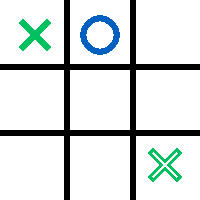
\includegraphics[scale=\scaling]{illustrations/board-notintelligent.pdf}%
\captionof{figure}{Η 2η κίνηση του έξυπνου χαρτιού (κάτω δεξιά) αν ο παίκτης με τα Ο παίξει σε πλευρικό τετράγωνο. Αυτή η κίνηση καταλήγει σε ισοπαλία, ενώ υπάρχει καλύτερη που οδηγεί αυτόματα στη νίκη.
%Το έξυπνο χαρτί ξεκινά παίζοντας σε μια γωνία. Αν ο παίκτης με τα Ο παίξει σε πλευρικό τετράγωνο τότε το έξυπνο χαρτί θα συνεχίσει παίζοντας στη διαγωνίως απέναντι γωνία. Έτσι όμως, θα οδηγήσει το παιχνίδι σε ισοπαλία, ενώ υπάρχει καλύτερη κίνηση που οδηγεί στη νίκη.
\label{fig:board-notintelligent}}}
έξυπνο χαρτί ξεκινά πάντα παίζοντας με τα Χ σε γωνιακό τετράγωνο. Αν ο παίκτης με τα Ο απαντήσει παίζοντας σ' ένα πλευρικό τετράγωνο (θέσεις \pyinline{1}, \pyinline{3}, \pyinline{5} και \pyinline{7}, σύμφωνα με την αρίθμησή μας) τότε το έξυπνο χαρτί θα επιλέξει τη γωνία που βρίσκεται διαγωνίως απέναντι από την αρχική (σχήμα \ref{fig:board-notintelligent}). Αυτή η κίνηση καταλήγει σε ισοπαλία, ενώ υπάρχει καλύτερη που οδηγεί με βεβαιότητα τον παίκτη με τα Χ στη νίκη.

Να επεκτείνετε τις οδηγίες του έξυπνου χαρτιού έτσι ώστε να μην παρουσιάζουν αυτή την ``αδυναμία''. Όταν ο παίκτης με τα Ο ξεκινήσει παίζοντας σε πλευρικό τετράγωνο, οι οδηγίες θα πρέπει να επιλέγουν την κατάλληλη κίνηση ώστε ο παίκτης με τα Χ να κερδίζει. Στη συνέχεια, να επεκτείνετε ανάλογα και τη συνάρτηση \pyinline{paperPosition}. 

\begin{note}Αν προτιμάτε να βρείτε έτοιμες τις τροποποιημένες οδηγίες, ώστε να εστιάσετε μόνο στην υλοποίησή τους, μπορείτε να ανατρέξετε στις επεκτάσεις του έξυπνου χαρτιού:
\href{http://pythonies.mysch.gr/ipaper-ext.pdf}{\url{pythonies.mysch.gr/ipaper-ext.pdf}}.
\end{note}
\solutionlink{oxo}{oxo-more-intelligent.py}
\end{exercise}

\begin{exercise}
Όταν φτάσαμε στο σημείο όπου το πρόγραμμά μας έπρεπε να αναλάβει το ρόλο ενός εκ των δύο παικτών, ήταν απαραίτητο να διαθέτουμε έναν μηχανισμό ο οποίος θα επέτρεπε στο πρόγραμμα να ελέγχει αν ένας παίκτης έχει τη δυνατότητα να κάνει τρίλιζα. Για τον σκοπό αυτό, αναπτύξαμε τη συνάρτηση \pyinline{checkPartial}.

Στο βιβλίο του \emph{Invent your own computer games with Python}, ο Al Sweigart αφιερώνει επίσης ένα κεφάλαιο στην τρίλιζα και προτείνει τον εξής τρόπο για να ελέγχεται αν ένας παίκτης έχει τη δυνατότητα να κάνει τρίλιζα: για κάθε διαθέσιμη θέση δημιουργείται ένα%
\marginnote{Για να δημιουργήσουμε ένα αντίγραφο μιας λίστας, μπορούμε να χρησιμοποιήσουμε τη μέθοδο \pyinline{copy()}, η οποία εφαρμόζεται σε μια λίστα κι επιστρέφει ένα αντίγραφό της.}
\emph{αντίγραφο} του πίνακα του παιχνιδιού, συμπληρώνεται η θέση με το σύμβολο του παίκτη και ελέγχεται αν έχει γίνει τρίλιζα. Ουσιαστικά, το πρόγραμμα \emph{δοκιμάζει} τι θα συμβεί στην επόμενη κίνηση.

Να αναπτύξετε μια νέα υλοποίηση της \pyinline{checkPartial} που να χρησιμοποιεί τη μέθοδο που περιγράψαμε για να ελέγξει αν ένας παίκτης έχει τη δυνατότητα να κάνει τρίλιζα. Για να ελέγχει η συνάρτησή σας αν μια κίνηση έχει οδηγήσει σε τρίλιζα, θα πρέπει να καλεί τη συνάρτηση \pyinline{check}.
\solutionlink{oxo}{oxo-lookahead.py}
\end{exercise}

\begin{exercise}
Μια %
\marginnote{\center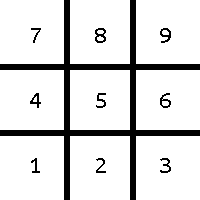
\includegraphics[scale=\scaling]{illustrations/board-user-dial.pdf}%
\captionof{figure}{Μια διαφορετική αρίθμηση των τετραγώνων της τρίλιζας, με βάση την οποία επιλέγει ο παίκτης το τετράγωνο στο οποίο θα παίξει. Αυτή η αρίθμηση αντιστοιχεί στο κλασικό αριθμητικό πληκτρολόγιο.\label{fig:board-user-dial}}}
αρίθμηση των τετραγώνων της τρίλιζας που πιθανώς να βόλευε περισσότερο τους παίκτες είναι αυτή που φαίνεται στο σχήμα~\ref{fig:board-user-dial}. Αυτή η αρίθμηση αντιστοιχεί στη διάταξη που έχουν τα αριθμητικά πλήκτρα σε ένα τηλέφωνο ή στο πληκτρολόγιο.

Τροποποιήστε το πρόγραμμα που αναπτύχθηκε έτσι ώστε ο παίκτης να επιλέγει το τετράγωνο στο οποίο θα παίζει με βάση αυτή την αρίθμηση.

\begin{note}
Μια πιθανή προσέγγιση είναι να τροποποιηθεί και η εσωτερική αναπαράσταση, ώστε να υπάρχει μια φυσικότερη αντιστοιχία με την αρίθμηση που αντιλαμβάνεται ο παίκτης. 
\solutionlink{oxo}{oxo-dial-representation.py}

Εναλλακτικά, μπορεί η εσωτερική αναπαράσταση να παραμείνει ως έχει και να προστεθεί στον κώδικα ένα επίπεδο ``αντιστοίχισης'' ανάμεσα στην εσωτερική αναπαράσταση και την αρίθμηση από την σκοπιά του παίκτη.
\solutionlink{oxo}{oxo-dial-mapping.py}
% [comment] Δώσε πιο συγκεκριμένες οδηγίες, που να ανταποκρίνονται και στις λύσεις που παρουσιάζεις. Π.χ. ποια είναι τα σημεία που αλλάζουν και με ποιο τρόπο;
% [comment] Σχολίασε τις λύσεις. Τόνισε ότι το κύριο πρόγραμμα δεν "βλέπει" και δεν ενδιαφέρεται για την αρίθμηση των τετραγώνων, όπως την αντιλαμβάνεται ο χρήστης, άρα εκεί δεν υπάρχουν αλλαγές. Δες αν έχει νόημα να διαφοροποιείς τις θέσεις (της λίστας) από τα τετράγωνα (του πίνακα του παιχνιδιού), είτε στα σχόλια, είτε στα ονόματα των μεταβλητών.
\end{note} 
\end{exercise}

\begin{exercise}
Το έξυπνο χαρτί παρέχει οδηγίες μόνο για λογαριασμό του παίκτη που παίζει πρώτος. Προσπαθήστε να γράψετε αντίστοιχες οδηγίες για τον παίκτη που παίζει δεύτερος και να τις υλοποιήσετε σε μια συνάρτηση αντίστοιχη της \pyinline{paperPosition}.

\begin{note}Αν προτιμάτε να βρείτε έτοιμες τις οδηγίες για τον δεύτερο παίκτη, ώστε να εστιάσετε μόνο στην υλοποίησή τους, μπορείτε να ανατρέξετε στις επεκτάσεις του έξυπνου χαρτιού:
\href{http://pythonies.mysch.gr/ipaper-ext.pdf}{\url{pythonies.mysch.gr/ipaper-ext.pdf}}.
\end{note}

Για να χρησιμοποιήσετε τη συνάρτησή σας, θα χρειαστεί να κάνετε τις απαραίτητες τροποποιήσεις ώστε το πρόγραμμα να μπορεί να αναλάβει το ρόλο οποιουδήποτε από τους δύο παίκτες.
\solutionlink{oxo}{oxo-twoplayer.py}
\end{exercise}

% [comment] Διαφορετικές εσωτερικές αναπαραστάσεις. Να εξεταστεί και μια αναπαράσταση όπου οι θέσεις είναι "συμβολικές" (πιθανώς σταθερές της μορφής upperLeft = 0)

%\vspace{24pt}
\vfill
%\fulllicensetrue
\sign{Γιώργος Μπουκέας, Βασίλης Βασιλάκης}{chapters/oxo.pdf}

\end{document}


%%%%%%%%

%\section{Ασκήσεις}

%\begin{exercise}
%\end{exercise}

%%%%%%%%

%\section*{}
%\vspace{4\parskip}
%\hrulefill

%\begin{theory}{}
%\end{theory}

%\hrulefill

%%%%%%%%%


